% Chapter 2

\chapter{Experiment} % Main chapter title

\label{Chapter2} % For referencing the chapter elsewhere, use \ref{Chapter2} 
%----------------------------------------------------------------------------------------
\section{The Large Hadron Collider (LHC) }\label{chapter2_sec1}
LHC is a particle accelerator of the world that has tendency to smash two protons beams at the energy up to 7.0~TeV each beam.
 It is the most advanced, complex and largest experiment in 
 the history of mankind, designed and constructed by a collaborative team of more than 10,000 technician, engineers and scientists from over 100 countries.
The LHC 
was constructed at CERN from 1998 to 2008, in a tunnel of 27~Kilometers (17 mi) circumference below the France-Switzerland border close to Geneva, Switzerland.
 The LHC is accommodated in a 3.8 meters wide  circular tunnel at a depth varies from 75-150 meters underground. Previously, this tunnel also bore Large Electron-Positron collider which was constructed from 1983 to 1988. 
 \par The first beam of protons was injected into LHC on September 10, 2008. The LHC was able to fire the protons around the tunnel in the segments of three kilometers each time. 
 The initial test to circulate the beams in clockwise and counterclockwise throughout the collider was also successfully completed by the same day. On 19 September 2008, 
 an electric defect triggered the magnet quench in about a hundred bending magnets. About six tonnes of liquid helium was lost due to which 50 superconducting magnets and their mounts were damaged. Three months later, CERN unfolded the details of the incident and published technical report. Particle accelerator
 was repaired  after this incident that took about an year. Finally, on November 20, 2009, LHC became operational again and a low energy beam was successfully rotated within
 tunnel. On November 30, shortly after, LHC became world's strongest particle accelerator after having achieved 1.18 TeV energy each beam thus defeating the Tevatron's highest achieved energy of 0.98~TeV. In 2010, 
 LHC kept boasting the beam energies and reached center of mass energy  up to 7~TeV (3.5~TeV each beam). In 2011 and then in 2012, LHC consistently delivered data at 7 and 8~TeV
 energies respectively. During 2013-14 , LHC machine was shutdown to do major parts upgrade on the LHC machine and detectors installed on it. In 2015, 
 upgraded LHC started again at 13~TeV close to full stipulated operating energies (14~TeV). After successfully delivering proton-proton collisions data during Run 2 till the end of 2018, LHC machine is shutdown for Long Shutdown 2 (LS2) upgrades and is expected be operational again for Run3 in 2021 after several upgrades. 
 
 %Since then, LHC is regularly delivering proton-proton collisions data to explore Higgs and other sectors of particle physics.
\begin{figure}
\begin{center}
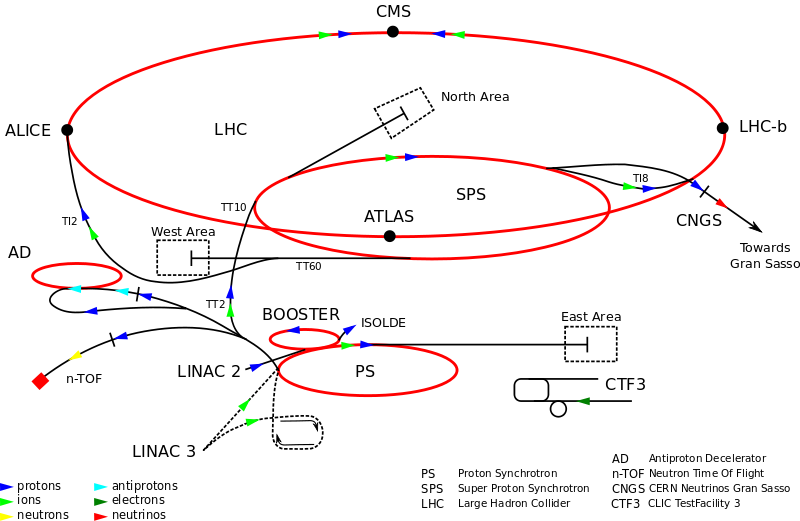
\includegraphics[width=0.8\linewidth]{Figures/chapter2_Figure/Cern-accelerator-complex.png}
\caption{LHC experiment at CERN}
\label{Fig:cern_accelerator_complex}
\end{center}
\end{figure}
\subsection{Machine Layout and Performance} 
\subsubsection{Machine Layout}
Basic layout of LHC and LEP  machines are similar, having eight linear and eight arcs sections as elaborated in Figure \ref{Fig:lhc_schematic_layout}~\cite{Reference28}. The LHC is 
designed to have two separate rings containing clockwise and counterclockwise proton beams, equipped with separate magnetic fields and vacuum chambers. These
two rings only intersect each other at the 
points where detectors are installed. Point 1 and point 5, opposite to each other, where ATLAS and CMS, two general purpose detectors of LHC, are installed respectively. The other 
two important detectors, ALICE and LHCb, are installed at point 2 and point 8 which are designed to study heavy ion Physics and B Physics respectively. Two protons beams are 
injected in the vertical plane in both rings close to point 2 and point 8. Among 8 sections, there are four with no beam crossing at all. Point 3 and point 
7 are equipped with two independent collimation systems for both rings. At point 4, two RF system are installed one for each beam. While at point 6, kicker 
magnets are installed to dump the beams.
\begin{figure}
\begin{center}

\includegraphics[width=0.8\linewidth]{Figures/chapter2_Figure/lhc-schematic.png}
\caption{The Schematic layout of the LHC}
\label{Fig:lhc_schematic_layout}
\end{center}
\end{figure}
\subsubsection{LHC Performance Goals}
LHC design goal is to test SM Physics to ultimate precision and hunt for any kind of new physics up to 14~TeV. Number of events (N) for a certain process produced at LHC are given as 
\begin{equation}
 N = \mathscr{L}\sigma_{process}
\end{equation}
\vspace{6em}

Here $\mathscr{L}$ represents machine luminosity and $\sigma_{process}$~ is the production cross section of a certain process. All possible processes' cross sections produced during proton-(anti) proton collisions at LHC machine luminosity $\mathscr{L} = 10^{33}~cm^{2}~s^{-1}$ are shown in Figure ~\ref{Fig:lhc_all}. 
Higgs production at LHC facility is rare as compared to other QCD and weak boson ($W,Z$) productions which act as backgrounds in the Higgs boson searches. In order to reconstruct
Higgs boson at LHC, one need to exploit specific final states providing enough signal to background discrimination. From Figure \ref{Fig:lhc_all} its clear that Higgs boson
production rises with increase in center-of-mass energies. So increase in  machine luminosity and center-of-mass energies enables us to get more 
statistics of Higgs boson. The Nominal luminosity for CMS and ATLAS experiment is $\mathscr{L}$ = 10$^{34}$cm$^{2}$s$^{-1}$, and nominal center of mass energy of LHC is $\sqrt{s} = 14$~TeV. 
 The cross section in Figure \ref{Fig:lhc_all} ~\cite{Reference29}~shows that LHC has possibility to produce a single Higgs boson after every 100~s at mass 500~GeV. To get 
ultimate number of Higgs bosons produced at certain luminosity, one need to multiply this with specific branching ratio, selection and reconstruction efficiencies. 
\subsubsection{Nominal Luminosity and Beam Parameters}
The machine luminosity can be expressed in terms of beam parameters as:
\begin{equation}
 \mathscr{L} = \frac{\gamma_{r}N_b^{2}f_{rev}n_{b}}{4\pi\epsilon_{n}\beta^{\ast}}F
\end{equation}

here $\gamma_{r}$ represents relativistic factor; however,  $N_{b}$ and  $n_{b}$ are the number of particles in a bunch and number of bunches in a beam respectively. While $\beta^{\ast}$ represents the 
beta function at the collisions point and F is the factor to account for geometrical depletion in luminosity due to cross angle at interaction point (IP). 
This factor can be written as below
\begin{equation}
 F = \left(1+(\frac{\theta_{c}\theta_{X}}{2\sigma^{\ast}})^{2}\right)
\end{equation}
where $\theta_c$, $\theta_z$ and $\sigma^{\ast}$ are crossing angle at point of interaction, root mean square (RMS) length of bunch and $\sigma^{\ast}$ the 
transverse RMS size of beam at IP. The expression above is valid for two circular beams with same parameters. \par The two major experiment of LHC, the CMS~\cite{Reference30} and the ATLAS~\cite{reference31}, are designed to operate at luminosity of $\mathscr{L} = 10^{34} cm^2s^{-1}$. 
The summary of the 
parameters to obtain this nominal luminosity is summarized in Table \ref{Tab:nominal_lumi_parameters}. Such high luminosity can not be attained by 
proton-anti-proton collisions, leaving
only possibility of proton proton collisions for LHC machine.  To align two opposite moving proton beams in both rings for collisions needs dipole 
magnetic with opposite fields 
direction. The LHCb~\cite{Reference32} detector is specially designed to study B Physics with peak luminosity $\mathscr{L} = 10^{32} cm^2 s^{-1}$. And the ALICE~\cite{Reference33} is the 
detector to study 
heavy-ion collisions targeting highest luminosity $\mathscr{L} = 10^{27} cm^2 s^{-1}$.
\begin{table}
\begin{center}
\caption{Parameters values to obtain LHC nominal luminosity for detectors.}
\label{Tab:nominal_lumi_parameters}
\begin{tabular}{ll}
  \hline
  Parameter & Value \\ \hline
  circumference & 26.7~km \\
  center of mass energy ($\sqrt{s}$) & 14~TeV \\
  Luminosity (nominal) & $10^{34} cm^2s^{-1}$ \\
  Bunch spacing & 25~ns \\
  distance between bunches & 7.5~m \\
  No. of bunches in ring & 2808 \\
  No. of protons in a bunch & $1.15\times 10^{11}$\\
  beta function at the collision point($\beta^{\ast}$)& 0.55~m \\
  Transverse RMS size of beam at impact point($\sigma^{\ast}$) & 16.3~$\mu$m  \\
  Magnetic field strength at 7~TeV(B) & 8.33~T \\
  Temperature of magnet (T)   & 1.9~K \\ \hline
\end{tabular}
\end{center}
\end{table}
\begin{figure}
\begin{center}
%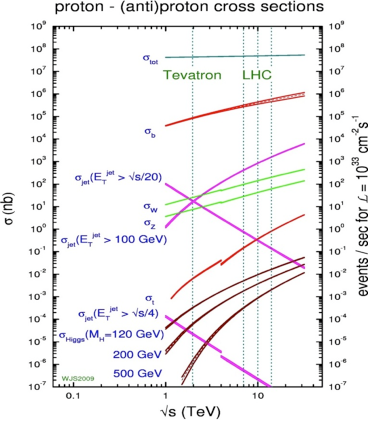
\includegraphics[width=0.8\linewidth]{Figures/chapter2_Figure/LHC_all.png}
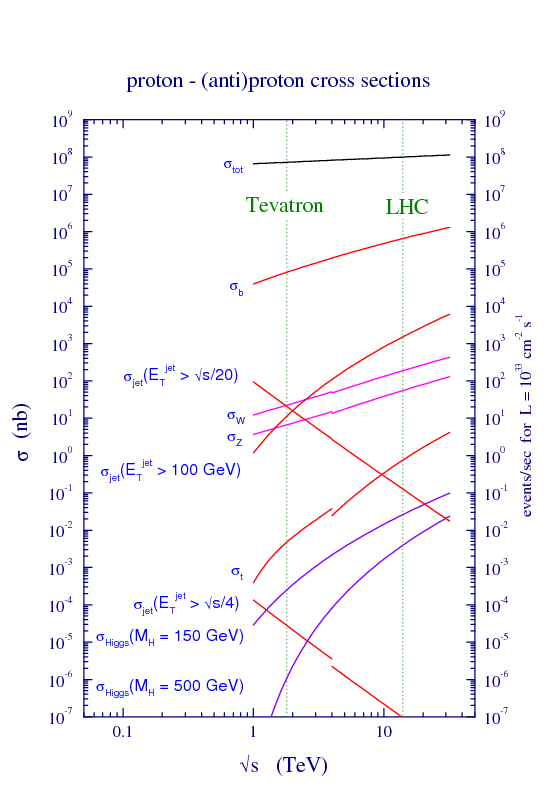
\includegraphics[width=0.8\linewidth]{Figures/chapter2_Figure/LHC_all2.png}
\caption{Cross section values for different process corresponding to machine luminosity $ \mathscr{L} = 10^{33}~cm^{2}~s^{-1}$.}
\label{Fig:lhc_all}
\end{center}
\end{figure}
%\subsection{Data Taking from 2010 to 2015}
\subsection{Data Taking from 2015 to 2018 (Full Run 2) }
%LHC started to deliver regular data from 2010. In 2010, LHC operated at 7~TeV center-of-mass energy with continuous increase in luminosity and  delivered 47
%\ipb proton proton collisions data. During 2011, LHC continued with 7~TeV center-of-mass energy with higher luminosity as compared to last year and delivered 
%6.1~\ifb~of data. Figure~\ref{fig:luminosity_2011} shows the LHC delivered and CMS recorded integrated luminosity throughout the year. LHC team decided to increase 
%center-of-mass of energy to 8~TeV during 2012 and luminosity reached at the value of $10^{33} cm^{-2}s^{-1}$. LHC delivered 23.3~\ifb of data during 2012 as 
%shown in Figure~\ref{fig:luminosity_2012}. The protons bunch spacing was reduced from 50~ns to 25~ns to increase the luminosity. 
After successful data taking during Run 1, LHC machine was shutdown for two years in 2013 and 2014 for major upgrades in LHC machine and detectors. LHC started again in 2015 at center-of-mass energies to 13~TeV(close to its design value i.e 14~TeV). LHC delivered 4.2~\ifb during 2015 at 13~TeV center of mass energy and subsequently, it delivered 41.0~\ifb, 49.8~\ifb and 67.9~\ifb  
during the years 2016, 2017 and 2018 as shown in the Figure \ref{fig:luminosity_2015}, \ref{fig:luminosity_2016}, \ref{fig:luminosity_2017} and \ref{fig:luminosity_2018} respectively. 
\vspace{6em}

%%%%%
\begin{figure}[!htb]
  \begin{center}
    \subfigure[]{
      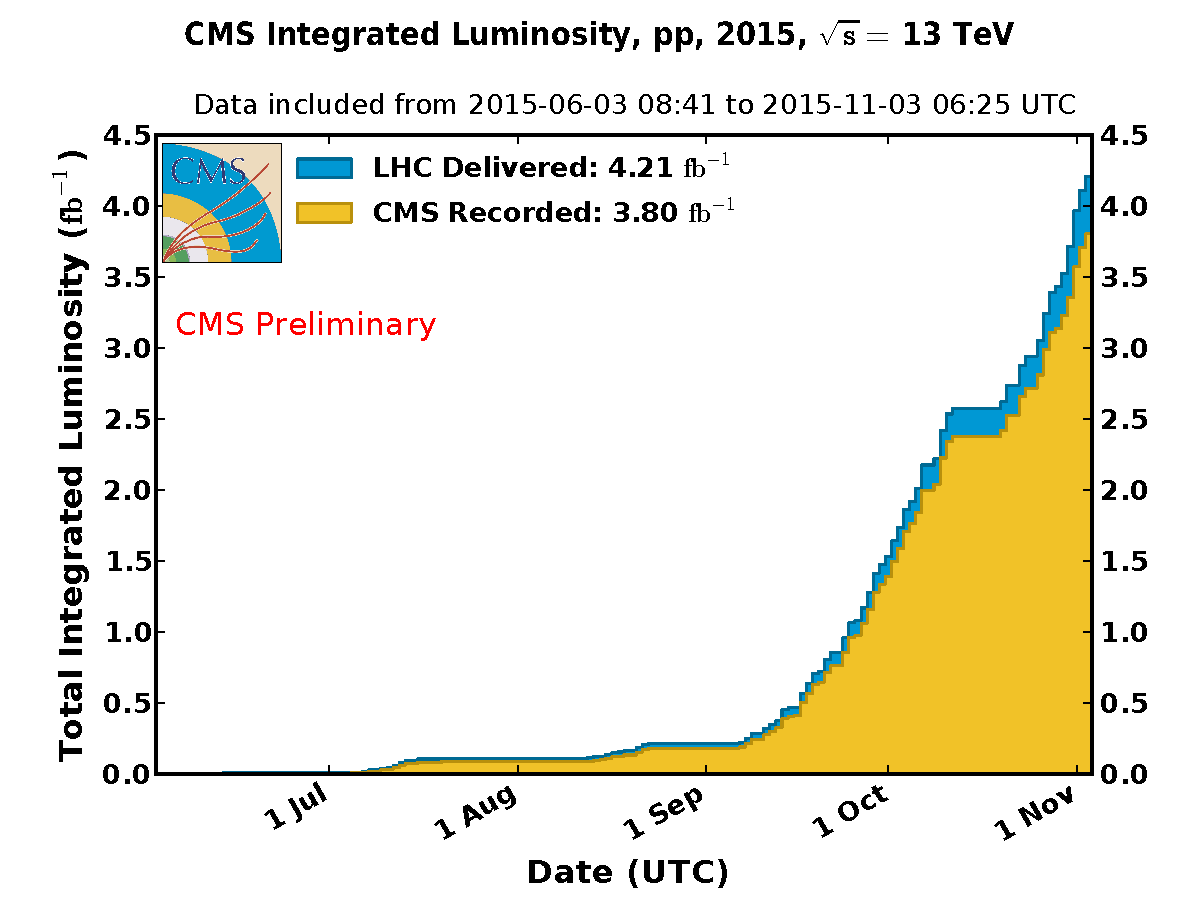
\includegraphics[width=0.48\textwidth,angle=0]{Figures/chapter2_Figure/int_lumi_per_day_cumulative_pp_2015_prelim.pdf}
      \label{fig:luminosity_2015}
    }
    \subfigure[]{
      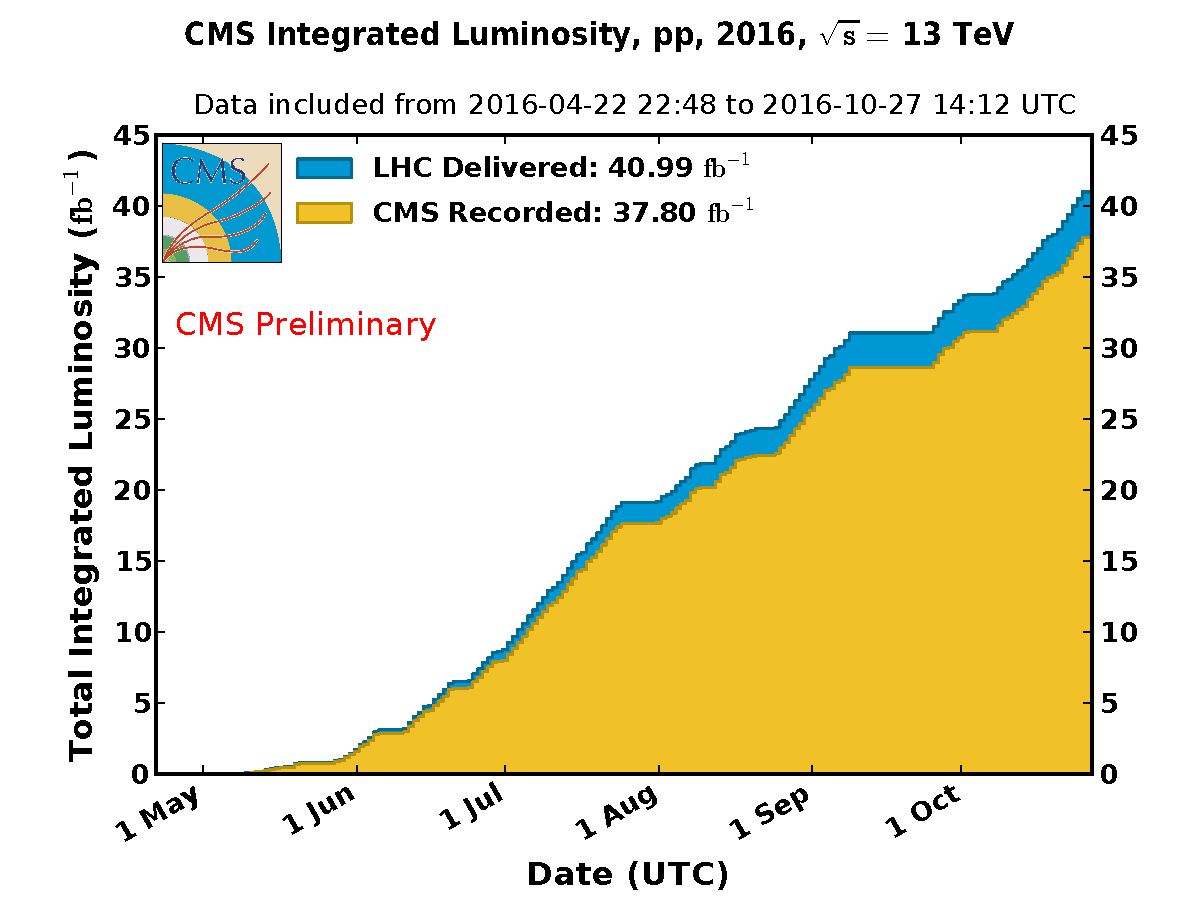
\includegraphics[width=0.48\textwidth,angle=0]{Figures/chapter2_Figure/int_lumi_per_day_cumulative_pp_2016_prelim.pdf}
      \label{fig:luminosity_2016}
    } 
    \subfigure[]{
      %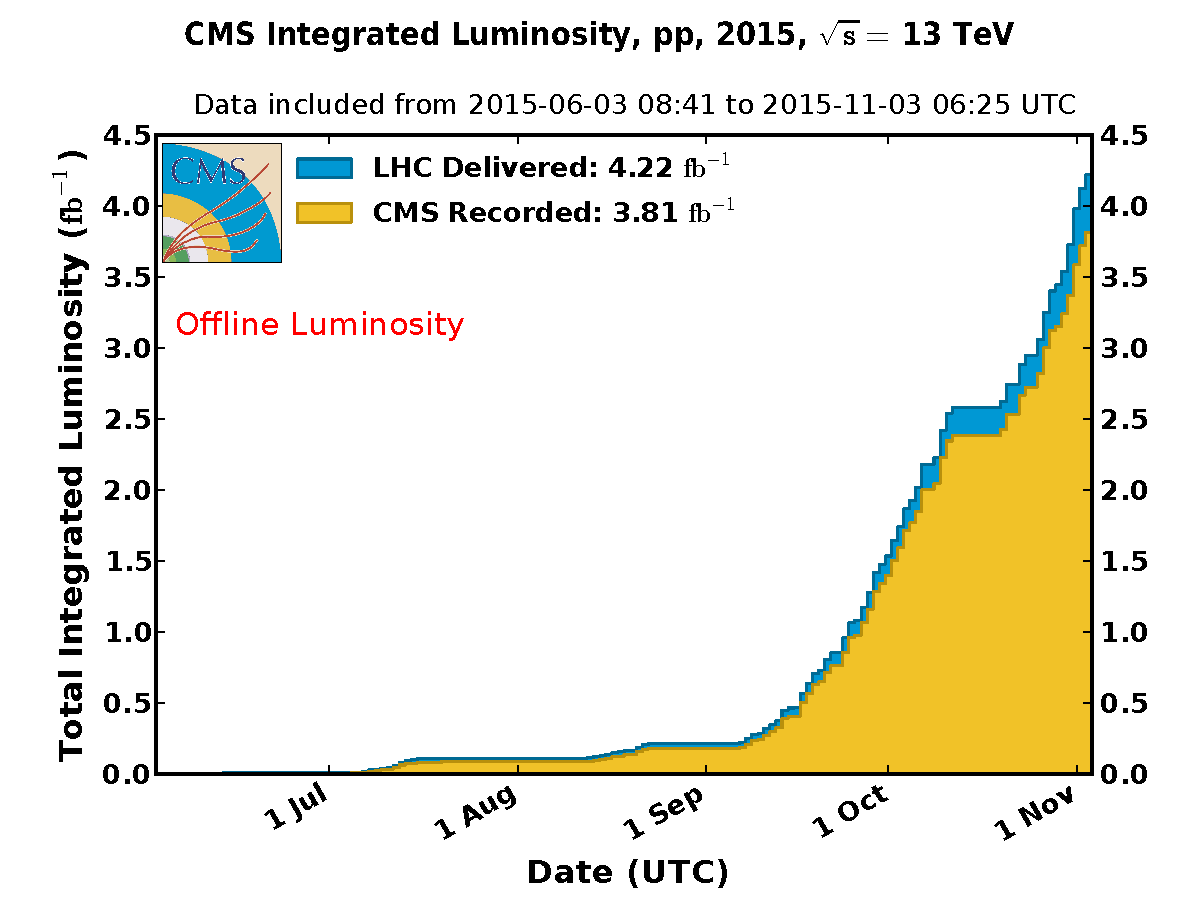
\includegraphics[width=0.48\textwidth,angle=0]{Figures/chapter2_Figure/int_lumi_per_day_cumulative_pp_2015.pdf}
      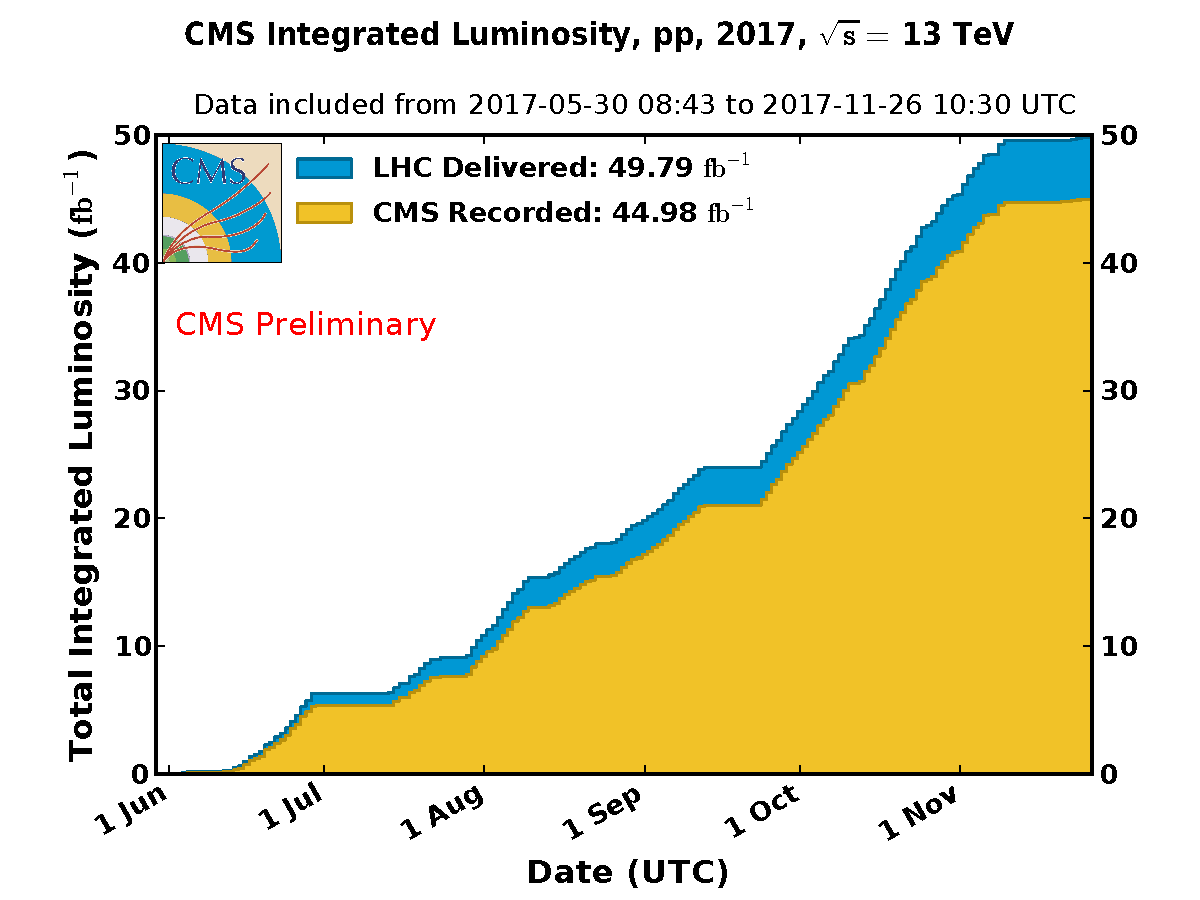
\includegraphics[width=0.48\textwidth,angle=0]{Figures/chapter2_Figure/int_lumi_per_day_cumulative_pp_2017_prelim.pdf}
      \label{fig:luminosity_2017}                                                                                                                            
    } 
    \subfigure[]{
      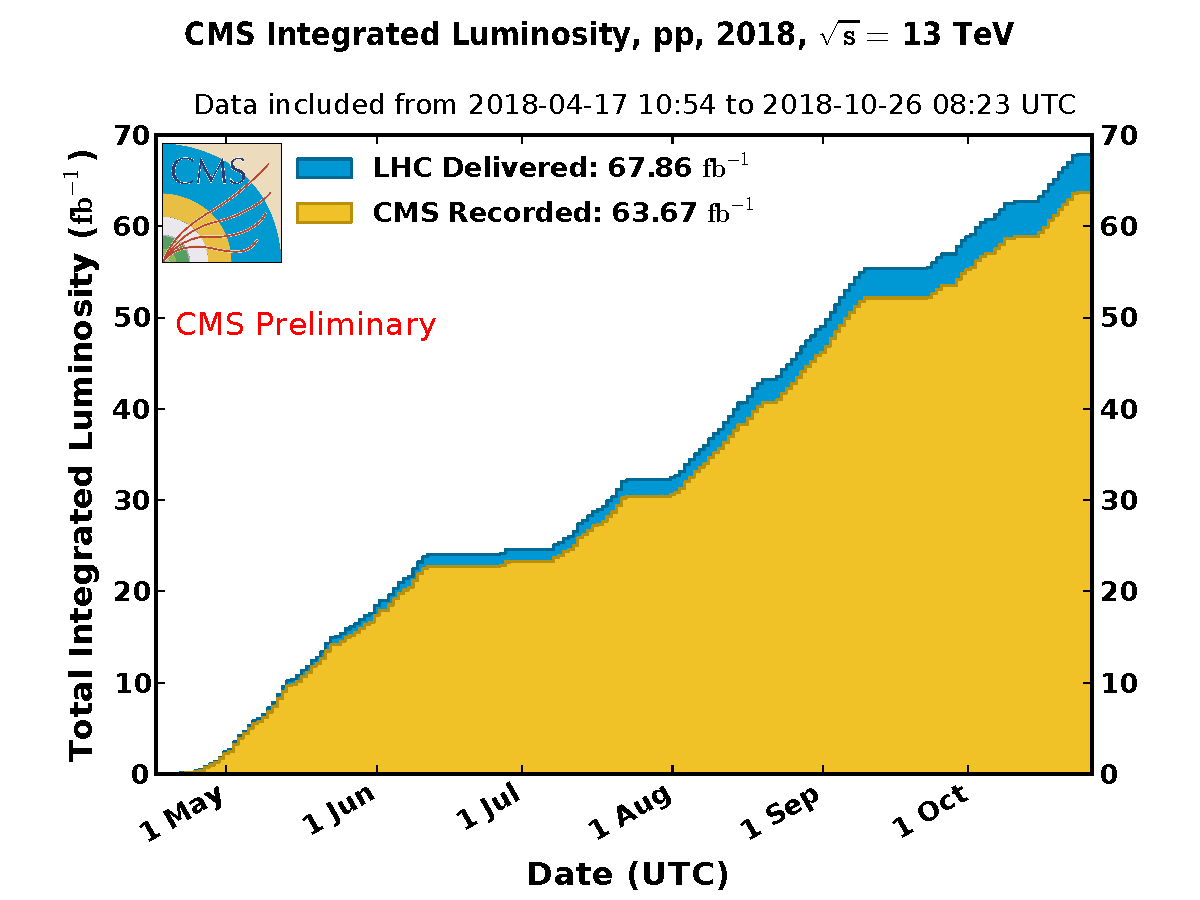
\includegraphics[width=0.48\textwidth,angle=0]{Figures/chapter2_Figure/int_lumi_per_day_cumulative_pp_2018_prelim.pdf}
      \label{fig:luminosity_2018}
    }\\
    \caption{Integrated luminosities of LHC delivered (blue) and CMS recorded (yellow) data for year 2015(a), year 2016(b), year 2017(c) and year 2018(d).}
  \label{fig:test}
\end{center}
\end{figure}
%==========================================================================================
\section{The Compact Muon Solenoid (CMS) Experiment}
The CMS detector is 28 m in length, 15 m in height and 14,000 tonnes heavy general purpose particle detector installed on LHC ring. It is capable to study large areas from SM Physics (including Higgs Physics) to search for extra dimensions and the dark matter. CMS is efficient 
enough to cover a large range of physics with energy ranges from a few 100~GeV to TeV scale~\cite{Reference34}. CMS and ATLAS experiment shares the same 
physics goal though both
independent experiment uses different technical solution and detectors design. It is apparent from Figure \ref{Fig:lhc_all} that the total cross section proton-proton collisionis at  $\sqrt{s} = 14 $~TeV is approximately 100~mb. While designed LHC luminosity leads to have $10^9$ inelastic events/s approximately. It is huge experimental challenge to deal with such high rate collisions. 
CMS trigger system helps to select online events and reducing the huge rate to approximately 100 events/s to be stored and used for physics analysis later. 
The read-out and trigger system designed to meet the short bunch crossing time, 25 ns. 
\\Being CMS as general purpose detector, followings are  the main requirements to fulfill physics goal of LHC:
\begin{itemize}
 \item Good resolution for muon identification and momentum over wide range of dimensions and determination of the charge on muons with ultimate precision with momentum up to 1~TeV.
 \item Healthy inner tacker reconstruction efficiency and resolution of charged particle momentum. Efficient trigger system and better discrimination of  $\tau$'s and b-jets.  
 \item Good dielectron and diphoton mass and energy resolutions. 
 \item Good dijet-mass and missing-transverse-energy (MET) resolutions . 
\end{itemize}
\begin{figure}
\begin{center}
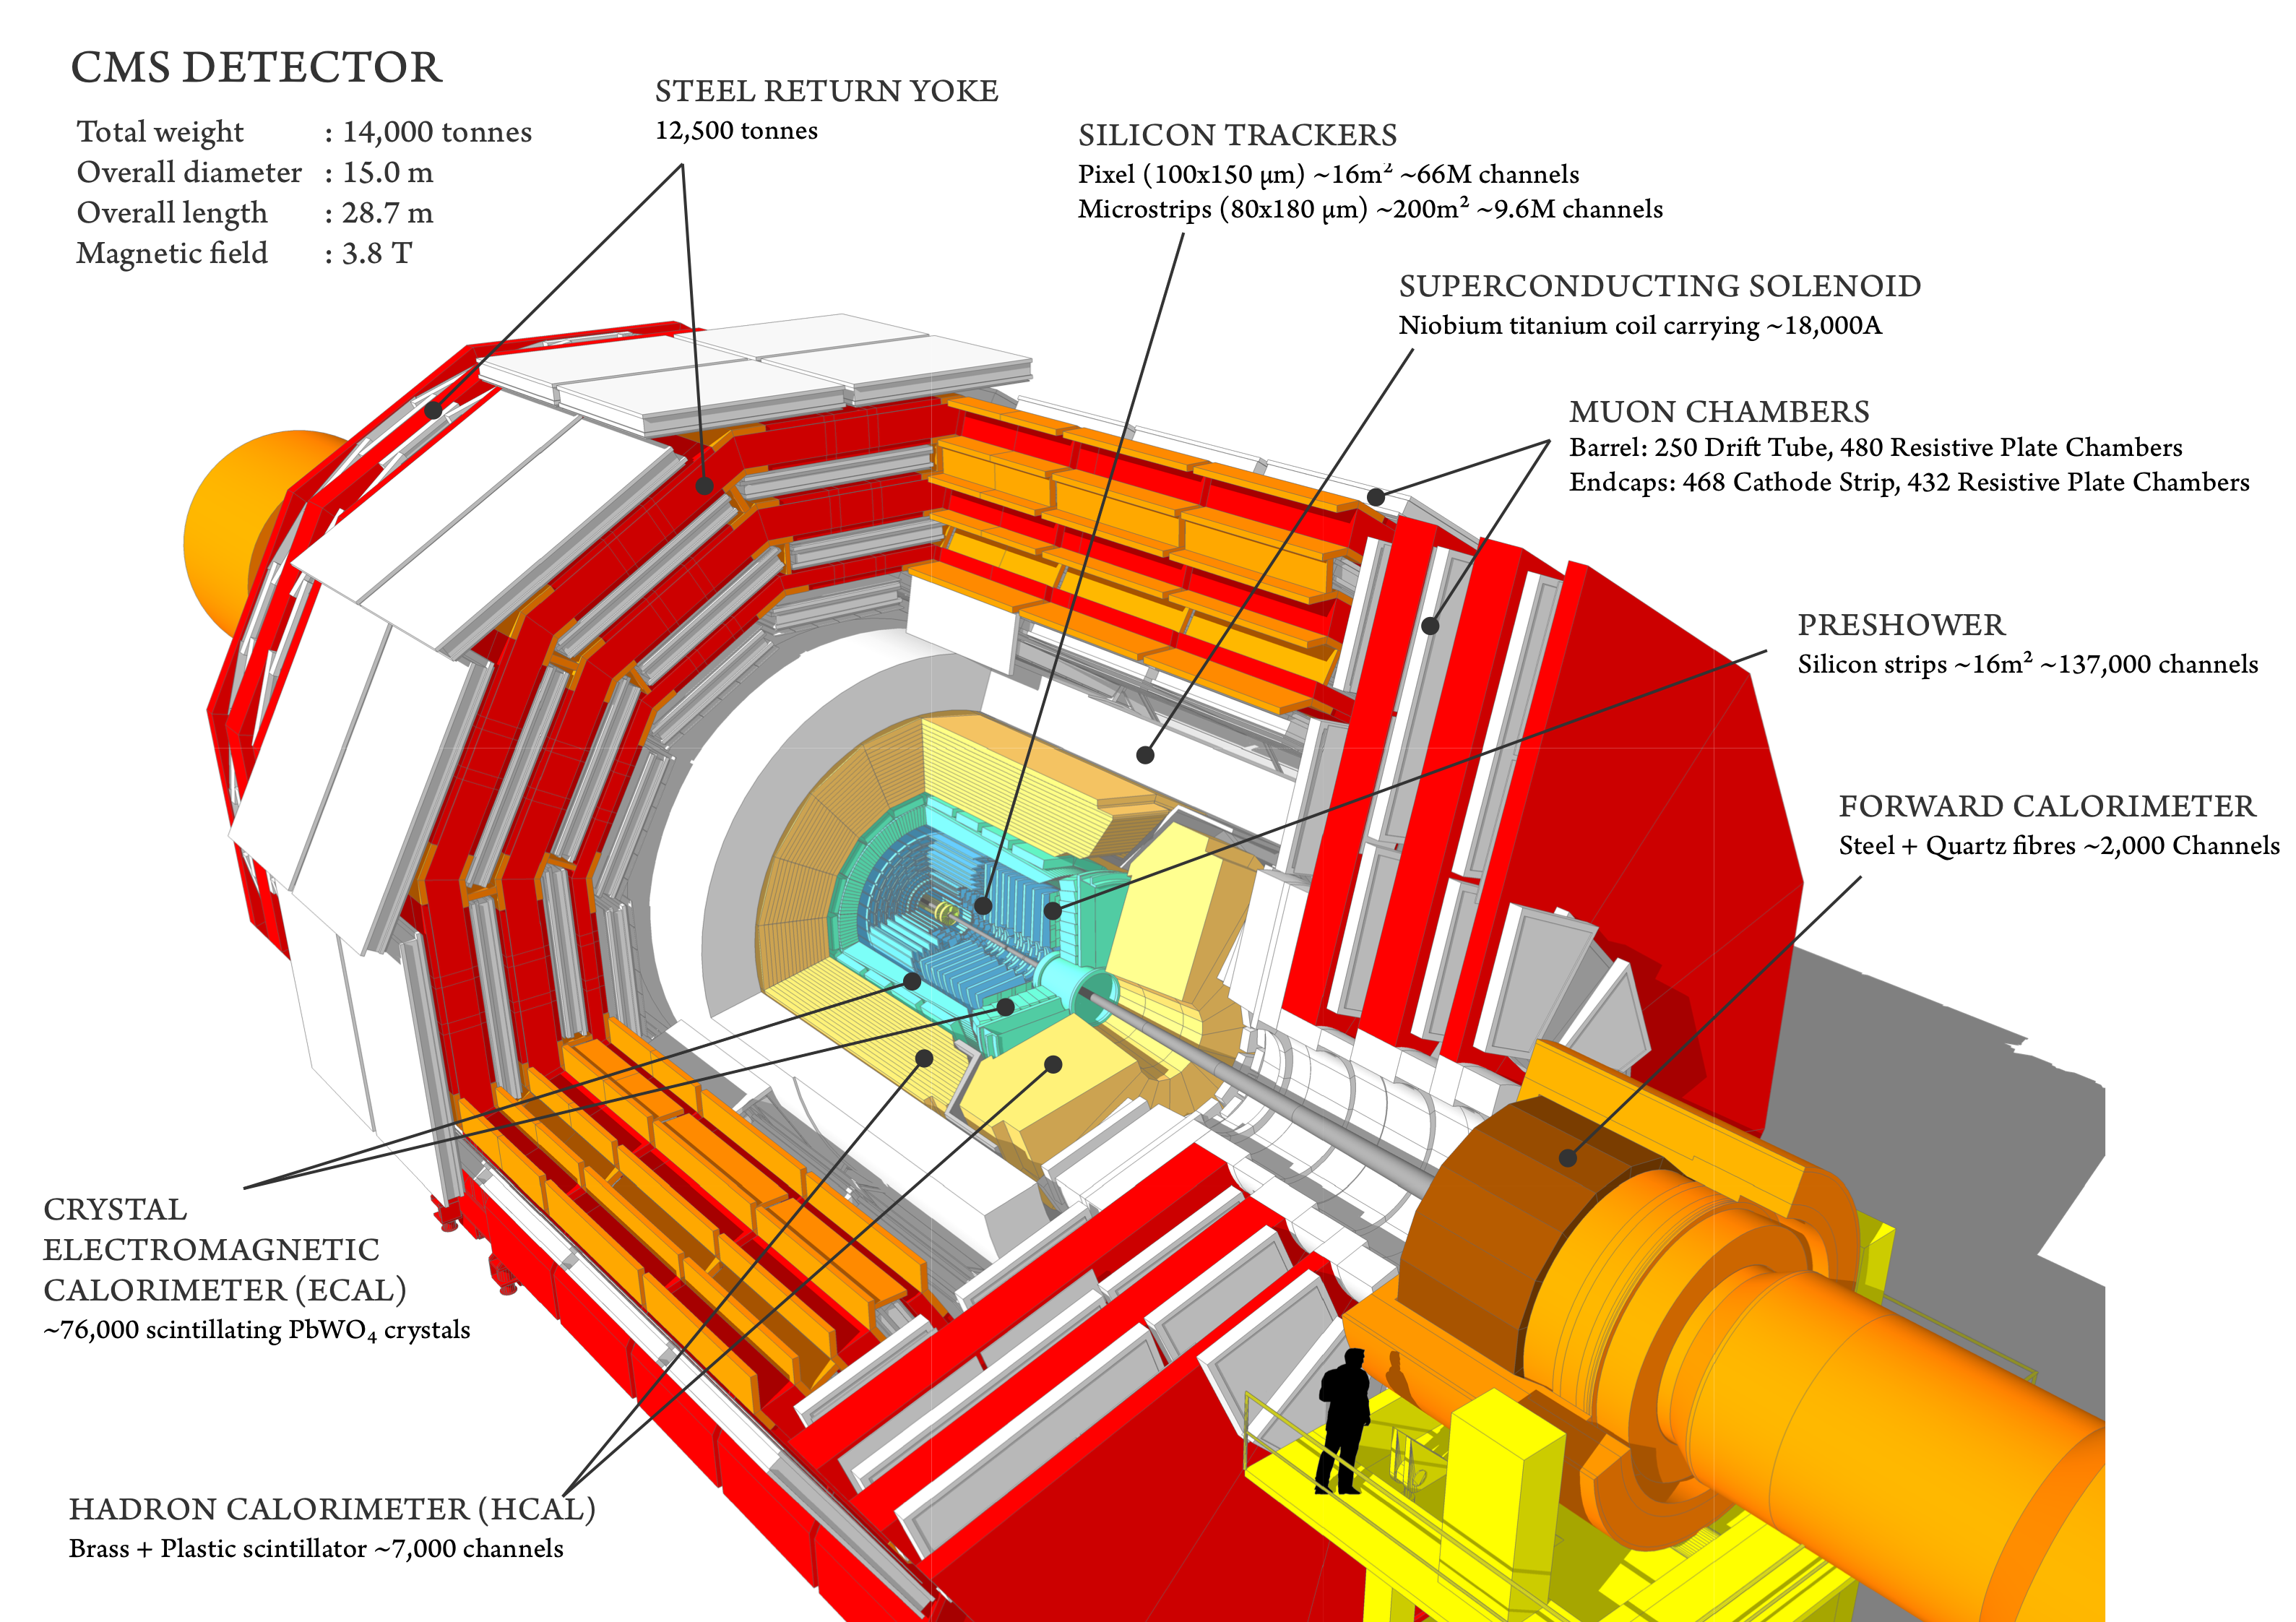
\includegraphics[width=0.8\linewidth]{Figures/chapter2_Figure/CMS_detector_design.png}
\caption{The CMS detector sectional view.}
\label{Fig:CMS_detector_design}
\end{center}
\end{figure}

Choice of magnetic field configuration is very important feature of a particle detector. Stronger magnetic field is needed to measure high energy 
charged particle momentum with precision. In CMS, this is achieved by selecting the superconducting magnets. \par
CMS overall  design is shown in Figure \ref{Fig:CMS_detector_design}. 
CMS magnet is superconducting solenoid which is 13m length with inner diameter of 6m. It is placed at the heart of CMS and is capable to produce a magnetic field of 3.8 T. The inner tracker system (ITS), electromagnetic calorimeter (ECAL) and hadronic calorimeter(HCAL) are the sub-detectors of CMS which are fitted inside the large solenoid magnet. Inner tracker of CMS have large track multiplicity as being closest to beam pipe where collisions happens. 
ECAL is build with crystals of lead tungstate which covers pseudorapidity up to $|\eta| < 3.0$. After ECAL, hadronic calorimeter is installed which is made of brass. Outermost layer of the CMS detector is the Muon System. Details of sub-detectors, trigger system and data acquisition systems will be described in next Sections. 
\subsection{CMS Detector Geometry}
The coordinate system would be described in this Section and will be used throughout. The CMS detector is like a closed cylinder around beam axis (Z axis)
as illustrated in Figure \ref{Fig:CMS_detector_design}. The center of the experiment lies inside beam pipe where two beams collides; the y axis is directed 
vertically upwards and the x axis being horizontal towards the LHC ring center.
\begin{figure}
\begin{center}

\includegraphics[width=0.8\linewidth]{Figures/chapter2_Figure/CMS_coorinidates.pdf}
\caption{The CMS Experiment coordinate system.}
\label{Fig:CMS_coordinates}
\end{center}
\end{figure}
The $r$ represents the radial component in transverse (xy) plane while $\phi$ is the the azimuthal angle measured from the x axis. $\theta$ is the polar angle which is measured from the z axis as shown in Figure \ref{Fig:CMS_coordinates}. Direction of any particle within CMS is described 
by $(\eta,\phi)$, where $\eta$ being the pseudo-rapidity defined as 
$\eta = -\ln \tan(\theta/2)$. LHC is colliding facility of protons mainly, which contains partons (i.e. quarks and gluons) carrying different fractions of proton's total 
momentum. As a results, events in CMS detector will have boosted center-of-mass as compared to lab frame along z axis. New defined quantity pseudorapidity  is invariant under 
these boosts. In short, pseudorapidity is approximation of rapidity in case of high energetic particles which are assumed to be massless and is defined below
\begin{equation}
 y = \ln(\frac{E+p_{z}}{E-p_{z}})
\end{equation}
\begin{equation}
 \approx \ln(\frac{1+\cos\theta}{1-\cos\theta)}
\end{equation}
\begin{equation}
 = \ln(\cot^{2}\theta).
\end{equation}
Pseudorapidity also helps to differentiate the barrel regions from the endcap regions of sub detectors. In terms of pseudorapidity, the barrel region are defined by 
$|\eta| < 1.5 $ whereas the endcap region corresponds to $1.5 < |\eta| < 3.0$. Formally, electromagnetic calorimeter and tracking system provides a coverage a region up to  $|\eta| < 2.5 $,
 while muon station covers up to $|\eta| < 2.4 $. So, in CMS muons and electrons are selected with $|\eta| < 2.4 $ and $|\eta| < 2.5 $ respectively. As there 
 is no transverse momentum (along y axis) before collisions which leads to have transverse momentum approximately zero.  The transverse energy of any particle 
 is orthogonal to z axis, defined as $E_{T} =  E \sin\theta$ and similarly the transverse momentum $p_T = p \sin\theta$. For a massless particle approximation, 
 electrons and muons, transverse momentum is equal to  transverse energy i.e. $E_T = p_T$.
 \\ As the CMS is hermetic, the energy of those particle which escaped from detector is understood as missing transverse energy. These particles
 can be new physics particles, neutrinos and neutralinos which have no or very little interaction with detector material.
\subsection{Inner Tracking System (ITS) }
 The CMS ITS is most inner sub-detector surrounding the beam pipe and region of interaction as shown in Figure \ref{Fig:CMS_detector_design}. Its is 2.5 m in diameter and 5 m in length feeding $|\eta|$ coverage up to 2.5.  The purpose of inner tracking system is to determine the trajectories of the charged particles needed to calculate their momentum and to reconstruct the secondary vertices. The whole ITS is placed in CMS solenoid under influence of a uniform magnetic field of strength 3.8 T. At LHC nominal luminosity of $10^{34} cm^2s^{-1}$, there is an average of more than 20 proton-proton interactions (for 2018 it was above 30) leading to average about 1000 
 particles emerging after every bunch crossing, 25 ns. To distinguish the trajectories and assign correct bunch crossing, fast response and high granularity
 detector technology is needed. To protect against radiation damage caused by intense particle 
 flux and priority to minimize the material to avoid from multiple scattering, nuclear reaction, bremsstrahlung and photon conversion, a compromise was 
 found to choose silicon detector technology. CMS inner tracker is made of about 200~$m^2$ of silicon hence being the largest tracker of its kind ever made. 
 \par CMS tracker detector should be robust  which can reconstruct tracks of charged particle in whole pseudorapidity range with momentum above 1~GeV to
 achieve LHC physics goals. Tracker also helps
 to identify other particles like electron, muons along with electromagnetic calorimeter. CMS inner operates under intense particle flux with hit
 density varies  from  1~MHz/mm${}^2$ at radial distance of 4cm decreasing to 60~KHz/mm${}^2$ and to 3~KHz/mm${}^2$ at distance of 115cm. 
 Keeping in view of hit densities, different types of detectors are installed at various radial distances of inner tracker listed in Table \ref{Tab:cms_detector_regions}. 
 Silicon detectors are chosen
 due its unique properties of fast response and good spatial resolution which enables it to work efficiently even in high radiation environment. To limit the damage mainly by 
 radiation the whole tracker system is kept at about -20$^{\circ}$ C.
\begin{table}
\begin{center}
\caption{Types of detectors installed in CMS tracking system.}
\label{Tab:cms_detector_regions}
\begin{tabular}{cccc}
  \hline
Section & Radial distance (cm) & Detector type & Cell size \\
\hline
Pixel   & $r<10$ & pixel & $100\mu m~\times150\mu m$ \\
TIB+TID & $20<r<55$ & microstrips & $10cm~\times150\mu m$\\
TOB+TEC & $55<r<110$ & strips & up to $25cm~\times180\mu m$\\
\hline
\end{tabular}
\end{center}
\end{table}
 %\par The CMS inner tracker schematic drawing is shown in Figure~\ref{Fig:CMS_tracker}~\cite{Reference34}. Tracker most inner region is the pixel detector that is nearest to the 
 \par The CMS inner tracker schematic drawing (as it stood before phase 1 upgrades) is shown in Figure \ref{Fig:CMS_tracker}~\cite{Reference34}. Tracker most inner region is the pixel detector that is nearest to the 
 interaction point consists of disk modules on each side and barrel layers. It provides accurate traces in $z$ and $r-\phi$ with a pixel cell of  size $100\times150\mu m^2$ covering the $|\eta|$ range up to 2.5. Pixel detector also plays its role for impact parameter resolution that helps to
 reconstruct secondary vertex ~\cite{Reference34}.
 Pixel detector delivers three spatial point with excellent precision throughout the coverage of pixel. % \ref{Fig:CMS_pixel}~\cite{Reference34}. 

 \par During data taking of Run 1 operations of LHC, some dynamic inefficiencies (about 5\% at an event pile-up of 40~)  were reported in the first layer of barrel of pixel sub-detector, due to the limited size of the readout
bandwidth. Subsequently, a new pixel detector was installed in March 2017 Ref. [see comment], equipped with one additional barrel  % The Phase-2 Upgrade of the CMS Tracker. Available online: https://cds.cern.ch/record/2272264 (accessed on 7 January 2019)
layer and one additional forward disk. In the new pixel detector, the innermost layer is closer to the
interaction point and the outermost one is further away from it as it is shown in Fig.  \ref{Fig:CMS_pixel_upgrade} %(Figure 1)
It also uses new Readout Chips (ROCs) benefitted from reduced data loss at higher collision rates with respect to Phase 1 operations (at 160 Mbit/s).
Bandwidth of the readout electronics was increased approximately by a factor of eight
(320 Mbit/s). In addition, DC-DC power converters were installed to allow reusing the existing fibers
and cables. Hence, the upgraded pixel detector has a higher rate capability and number of channels,
providing increased tracking efficiency, reduced fake rate, and improved impact parameter resolution.
In the figure \ref{Fig:hit_efficiency_upgrade} clear improvments in the dynamic efficiency of 2017 (with pixel upgrades) with respect to the 2016 (without pixel upgrades) can be seen.
%Overall, the pixel detectors is of 1~$m^2$ size containing 66 million pixels.  % to be updated ?? 

Silicon Strip is the second layer detector after pixel detector which is installed at  radial distance  from 20cm to 116cm.  This detector surrounds both sides of pixel with its tacker inner barrel (TIB) and
 inner tracker disk (TID) regions. There are 3 disks on each endcap and 4 barrel layers where silicon microstrips of thickness $320\mu$m are installed. Microstrips
 are aligned along with beam axis in the barrel region and in radial direction on disks. The strip pitch in barrel region varies  from 80$\mu$m to 120$\mu$m
 from inner to outer barrel layer. In the endcap region strip pitch changes from 100$\mu$m to 141$\mu$m. Finally, the most outer part of CMS tracker system 
 is tracker outer barrel (TOB) installed at radial distance from 55cm to 116cm containing 500$\mu$m thick 6 barrel layers with strip pitch of 183$\mu$m and 122$\mu$m. 
 TOB provides z coverage up to 118 cm, beyond this point 9 disks of tracker endcaps (TEC+, TEC-) are located that covers 124 cm$<|z|<$282 cm and 22.5 cm$<|r|<113.5$ cm.
\begin{figure}
\begin{center}

\includegraphics[width=0.8\linewidth]{Figures/chapter2_Figure/CMS_tracker.pdf}
	\caption{Schematic diagram of CMS tracker system. Lines represent detector modules (before phase 1 pixel upgrades ).}
\label{Fig:CMS_tracker}
\end{center}
\end{figure}
 \begin{figure}
\begin{center}
%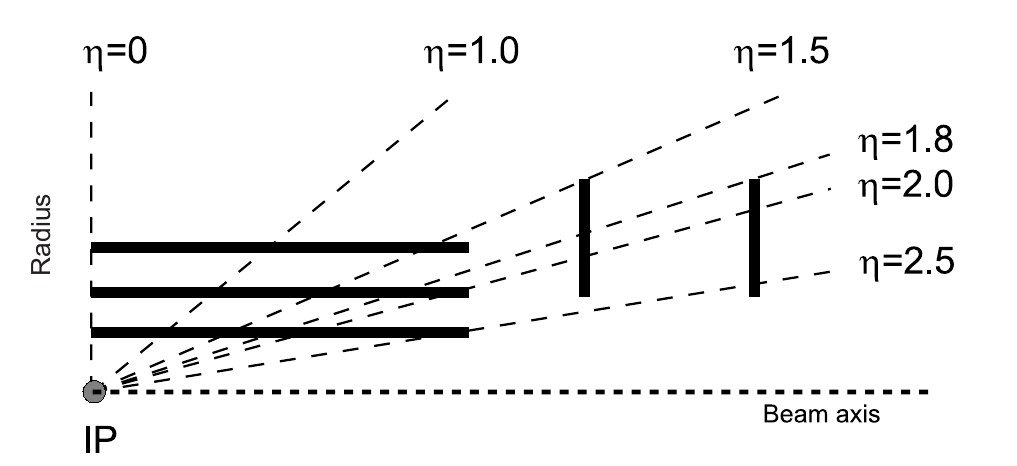
\includegraphics[width=0.8\linewidth]{Figures/chapter2_Figure/rename.png}
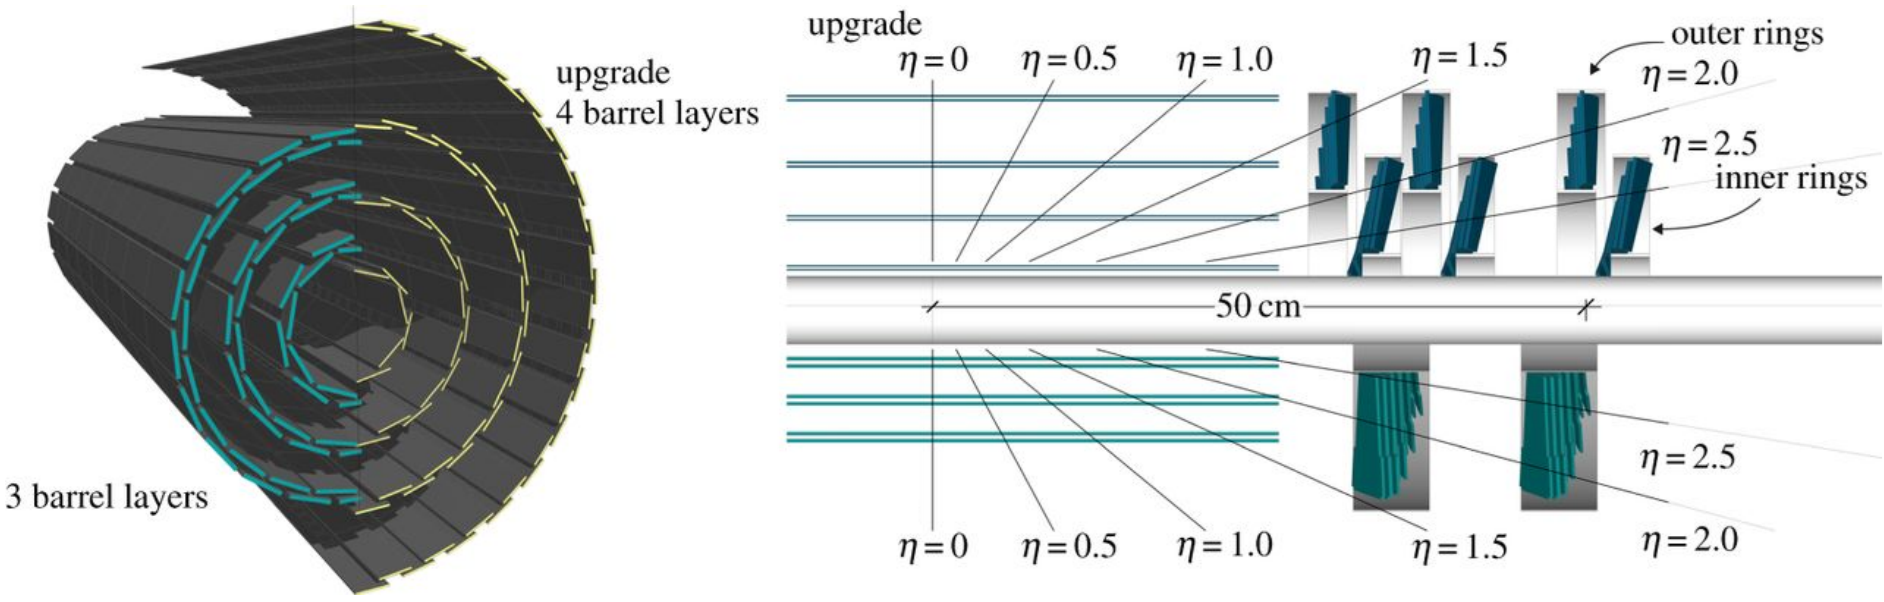
\includegraphics[width=0.8\linewidth]{Figures/chapter2_Figure/CMS_pixel_upgrade.png}
%\caption{CMS pixel detectors and hit coverage. Lines represent detector modules.}
\caption{Schematic diagram of pixel detector's upgrade. Old pixel detector is shown by the lower half detector, and the new pixel detector is represented by the upper half.}
\label{Fig:CMS_pixel_upgrade}
\end{center}
\end{figure}
\par To measure the  momentum in CMS tracker, we simply exploit the property of the charged particles to bend in the magnetic field. High momentum particles
will bend less in detector and vice versa, making resolution worse due to less curvature. 
\par The upgraded pixel detector improved $\Hllll$ analysis as there was significant increase in lepton number in an event thus improving the reconstruction of Z candidates and hence an increase in the selection efficiency upto much extent. [Ref. CMS-TDR-011]
\begin{figure}
\begin{center}
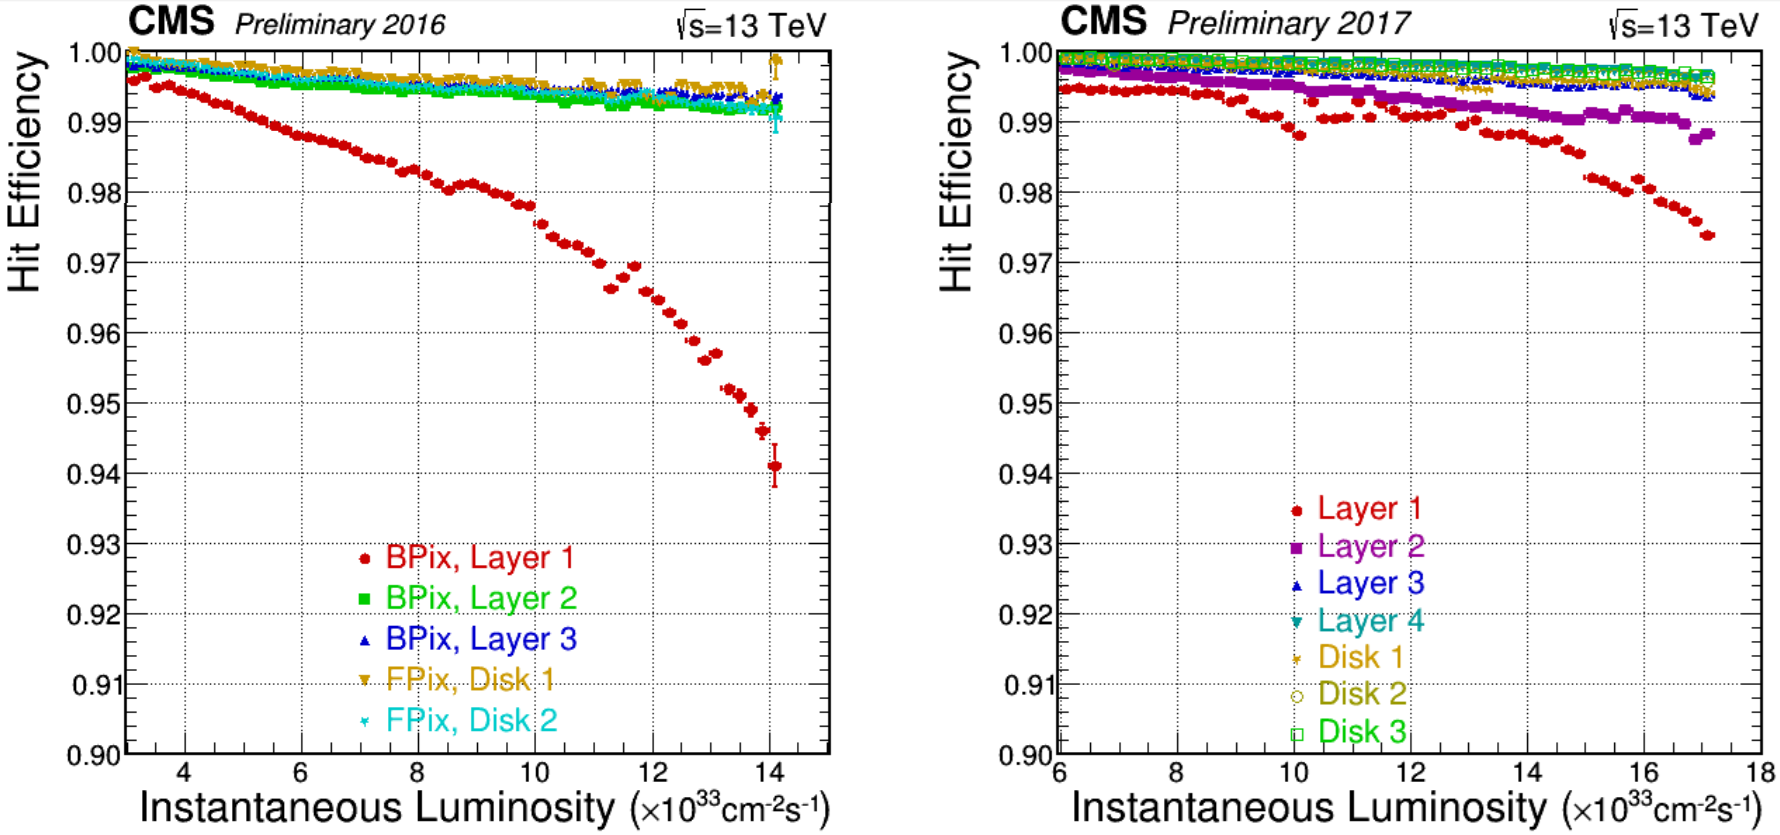
\includegraphics[width=0.8\linewidth]{Figures/chapter2_Figure/hit_efficiency_upgrade.png}
%\caption{CMS pixel detectors and hit coverage. Lines represent detector modules.}
	\caption{Pixel detector's hit efficiency as function of instantaneous luminosity corresponding to 2016 data (left) and to 2017 data (right) Ref. ~\cite{Sonneveld:2018ntf} %[in comments] }  % Sonneveld, J. Commissioning and first results from the CMS phase 1 upgrade pixel detector. In Proceedings of the 26th International Workshop on Vertex Detectors, Las Caldas, Asturias, Spain, 10–15 September 2017; PoS(Vertex 2017)018.
\label{Fig:hit_efficiency_upgrade}
\end{center}
\end{figure}

%The material in radiation length's for different sub detectors and functional modules are shown in Figure~\ref{Fig:CMS_tracker_material}~\cite{Reference34}. As in tracker, strips and pixel sizes are not uniform with 
%the variation of $\eta$, Figure~\ref{Fig:CMS_tracker_expected_efficiency}~\cite{Reference34} shows the expected performance of muon tracks resolution with $p_T$= 1, 10 and 100~GeV as function
% of $|\eta|$. While Figure~\ref{Fig:CMS_tracker_global_efficiency}~\cite{Reference34} shows  comparison of global track reconstruction efficiencies of muons and pions with 
% same transverse momentum. 
%\begin{figure}
%\begin{center}
%
\includegraphics[width=0.8\linewidth]{Figures/chapter2_Figure/tracker_meterial.pdf}
%\caption{Material in radiation length's for different sub detectors (left) and for different functional modules (right) as function of $\eta$}.}
%\label{Fig:CMS_tracker_material}
%\end{center}
%\end{figure}
% \begin{figure}
%\begin{center}
%
\includegraphics[width=0.8\linewidth]{Figures/chapter2_Figure/expected_efficiency.pdf}
%\caption{Expected single muons tracks resolution of transverse momentum (left), transverse impact parameter (middle) and longitudinal impact parameter (right)
%of $p_T = $ 1, 10, 100 GeV.}
%\label{Fig:CMS_tracker_expected_efficiency}
%\end{center}
%\end{figure}
%\begin{figure}
%\begin{center}
%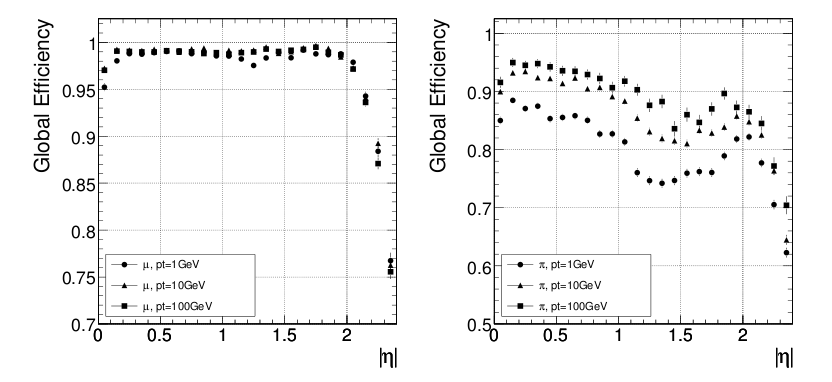
\includegraphics[width=0.8\linewidth]{Figures/chapter2_Figure/global_efficiency.png}
%\caption{CMS tracker global efficiency of muons (left) and pions (right) of $p_T = $ 1,10, 100 GeV.}
%\label{Fig:CMS_tracker_global_efficiency}
%\end{center}
%\end{figure}
\subsection{Electromagnetic Calorimeter (ECAL) }
ECAL is the cylindrical shaped, hermetic and homogeneous calorimeter build with crystals of lead tungstate (PbWO${}_4$). Its barrel ergion (EB) provides pseudorapidity coverage of $|\eta| < 1.479$ and contains 61200 PbWO${}_4$ crystals. Endcap region of the ECAL
(EE) provides pseudorapidity coverage up to $\eta < 3$ and is build with 7324 crystals on either side in endcap regions. The region of $1.4442 < |\eta| <1.56$ is regarded as crack region between barrel and endcaps as shown in Figure \ref{Fig:CMS_ECAL_layout} ~\cite{Reference34} is excluded for 
 physics analysis. A preshower detector is installed
in endcap regions to distinguish between single and diphoton close to each other e.g neutral pion decay 
($\pi^{\circ} \rightarrow \gamma\gamma $). Specially designed Avalanche photodiodes (APDs) and the Vacuum phototriodes (VPTs) are employed in barrel and endcaps region respectively ensure efficient working under high magnetic field. Higgs discovery (both in $H\rightarrow \gamma\gamma$ and $H \rightarrow ZZ \rightarrow 4\ell$ channels) is based on one of the ECAL key feature in the  design is to reconstruct
electrons and photons with high resolution. 
%enabled us to discover Higgs boson in both $H\rightarrow \gamma\gamma$ and $H \rightarrow ZZ \rightarrow 4\ell$ favorable channels. 
\subsubsection{ECAL Crystals and Geometry}
To make a compact and high granularity calorimeter which could fit inside the CMS solenoid, lead tungstate was the best option which is denser than
steel (8.28 g/cm${}^{3}$) with short radiation length (X_$\circ$) of 0.89~cm~\cite{cms:ECALTDR}. The scintillator (PbWO${}_4$) emits light which is directly proportional to incident particle's energy through ionization. Fast response  (same order of LHC bunch cross crossing i.e. 25ns) of PbWO${}_4$ makes it ideal for 
ECAL. In barrel region, there are 8.14 m${}^3$ active crystals  installed weighting up to 67.4 tonne. The each crystals cross section is measured to be 
22~$\times$~22 mm${}^{2}$ in barrel and 28.62~$\times$~28.62 mm${}^{2}$ at endcaps. 
Crystal length in barrel and endcaps is 230mm and 220 mm which is 25.8 and 24.7 times of the radiation length. 
\par The amount of emitted light from scintillator and amplification of photodiodes both are temperature dependent. The nominal temperature at which ECAL operates is around 18${}^{\circ}$C. 
For this reason, cooling system has been installed in ECAL to maintain the temperature at nominal value. The cooling system rotates water at
18${}^{\circ}$C through parallel grid of aluminium pipes a to maintain the temperature in the detector. In the barrel region, each supermodule has its independent
supply of water. The cooling system of  the ECAL work efficiently  and maintain the temperature of $18\pm0.05^{\circ} C$.

\begin{table}[!htpb]
\caption{ECAL crystal details at endcaps and barrel regions.}
\label{Tab:ecal_crystal_barrel_endcap}
\begin{tabular}{lll}
                   & Barrel & Endcaps \\
\hline
                   Number of crystals & 61200 & 14648 \\
 Crystal cross section in ($\eta,\phi$) & $0.0174 \times 0.0174$ & variable \\
 Cross section of front face of crystal & $22 \times 22 mm^2$ & $28.62 \times 28.62 mm^2$ \\
 Cross section of rear face of crystal & $26 \times 26 mm^2$ & $30 \times 30 mm^2$ \\
 Crystal length 		       & 230 mm & 220 mm \\
 Crystal length(in terms of $X_{\circ}$) & 25.8$X_{\circ}$ & 24.7$X_{\circ}$ \\
 \hline
 
\end{tabular}
\end{table}

\begin{figure}
\begin{center}

\includegraphics[width=0.7\linewidth]{Figures/chapter2_Figure/CMS_Electromagnetic_calorimeter.pdf}

\includegraphics[width=0.7\linewidth]{Figures/chapter2_Figure/ecal_2.pdf}
\caption{CMS ECAL layout and pseudorapidity coverage.}
\label{Fig:CMS_ECAL_layout}
\end{center}
\end{figure}

\subsubsection{Photodetectors}
The requirements on photodetectors are to be fast, robust and able to work efficiently in a region that contains 3.8 T magnetic field. Considering these requirements, different types
of photodetectors are installed both in the barrel and the endcap regions. In the barrel region, each crystal a pair of avalanche photodiodes are mounted with of 5~$\times$~5~mm$^{}^{2}$ active area. Gain of the working APD is 50 and in parallel read out. 
%page 35 ?
In endcap region, a specially designed vacuum phototriodes at National Research 
Institute Electron(St. Petersburg) for CMS ECAL was used. These are single gain photomultipliers with mean gain being 10.2~ in absence of field. The diameter of each VPT is 22mm.  The total
active area is almost 280mm${}^2$ where one VPT is attached at the back of every crystal. Their fine coper anode makes them capable to work under 
intense magnetic field. As compared to APDs, VPTs have lower quantum efficiency and the internal gain which is balanced out with the larger
back face crystal coverage. The summary of number of the crystals with their dimensions are summarized in Table \ref{Tab:ecal_crystal_barrel_endcap}.
\subsubsection{Preshower}
\par Purpose of the installation of preshower detector is the identification of neutral pions detected in the endcaps regions. Due to its high granularity, the preshower helps to differentiate between electron and minimum ionizing particles (MIPs) and to determine the position of electrons and photon. It provides the pseudorapidity coverage of $1.653<|\eta|<2.6$. 
\subsubsection{Energy Resolution}
It can defined as  
\begin{equation}
 \left(\frac{\sigma}{E}\right)^{2}= \left(\frac{S}{\sqrt{E}}\right)^{2}+\left(\frac{N}{E}\right)^2+C^2
\end{equation}
where C is the constant of proportionality and is extracted by fitting the measured points to the function, N being noise term and S is stochastic term. 
%A measurement of energy resolution has been made by using electron of energies from 20 to 250~GeV in test beam~\cite{Reference35}. The measurement was made by considering arrays of $3\times 3$ or $5 \times 5$. No correlated significant noise was observed in these arrays. The measurements summary is shown in 
Recently relatively energy reslution study of ECAL using 2017 data and MC has been performed using Z events decaying to a pair of electrons. The resolution plots for bremsstrahlung electrons ($R_{9}$>0.94 and $R_{9}$<0.94) is separately shown for data and MC in the Figure \ref{Fig:CMS_ECAL_energy_resolution}~\cite{Zghiche_2019}.  % https://iopscience.iop.org/article/10.1088/1742-6596/1162/1/012001/pdf 
For $\Hllll$ analyses, excellent energy resolution for leptons is important for precise measurements for which ECAL of CMS plays an important role.
\begin{figure}
\begin{center}
%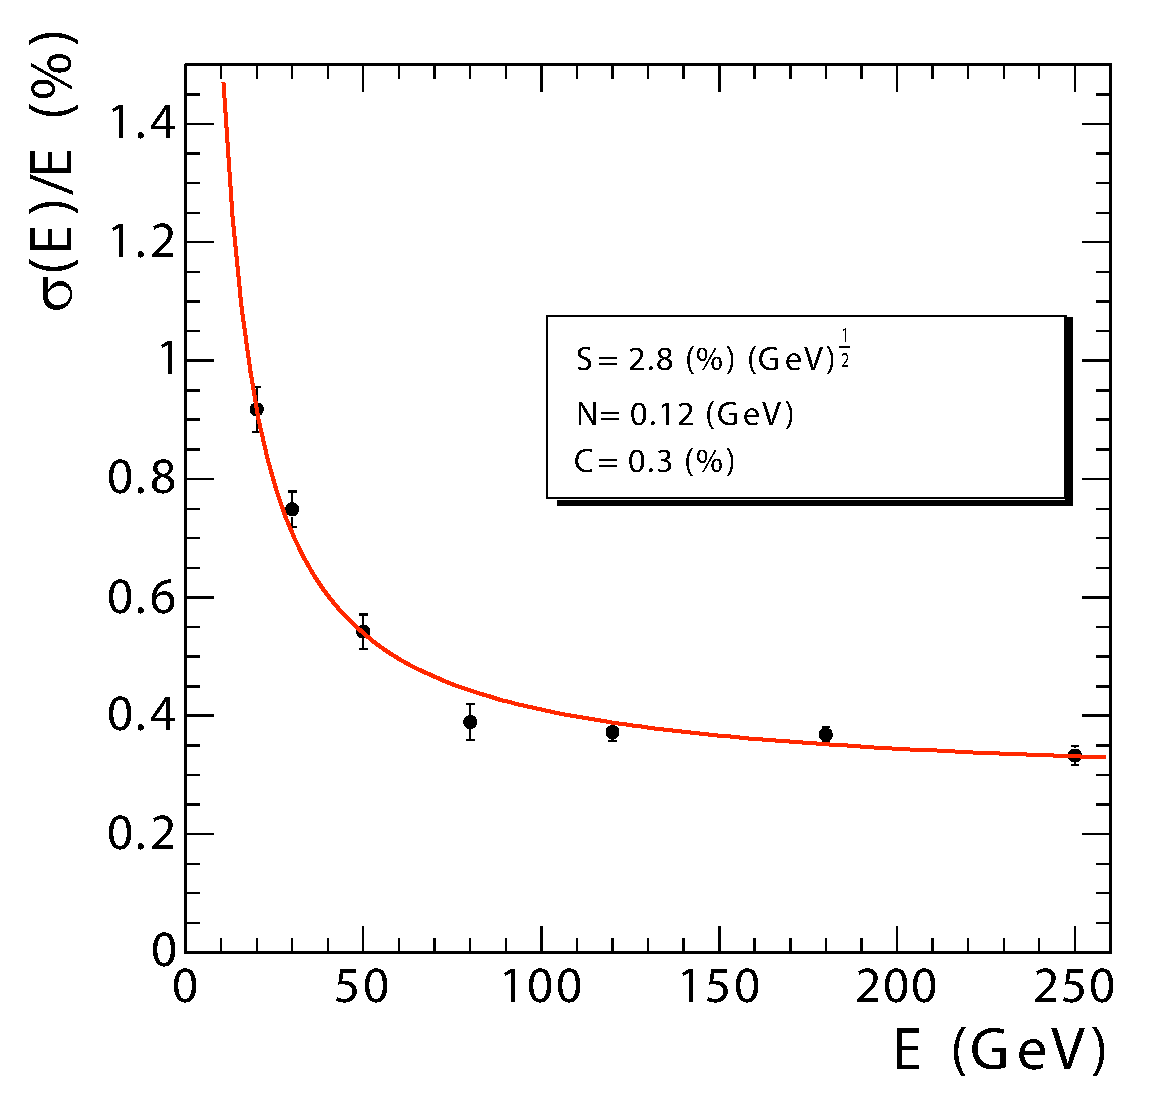
\includegraphics[width=0.7\linewidth]{Figures/chapter2_Figure/ecal_energy_resolution.pdf}
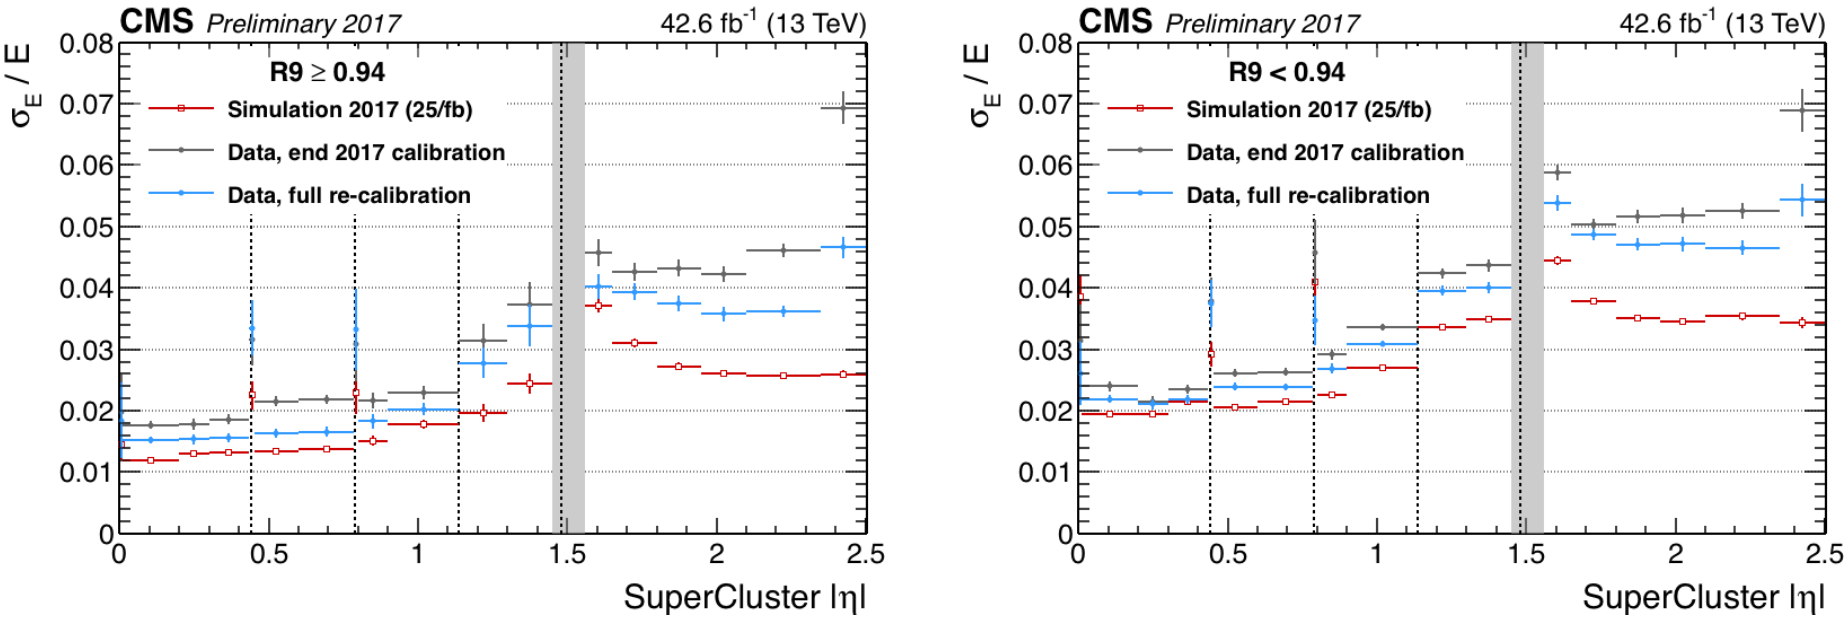
\includegraphics[width=0.85\linewidth]{Figures/chapter2_Figure/ecal_energy_resolution_2017.png}
\caption{CMS ECAL energy resolution.}
\label{Fig:CMS_ECAL_energy_resolution}
\end{center}
\end{figure}
%start from page 36


\subsection{Hadron Calorimeter}
CMS being a general purpose detector is capable to study several final state signatures involved in a large range of high energy processes. The hadron 
calorimeter (HCAL) provides the measurement of energies and positions of hadronic jets (for example neutrons, protons, kaons and 
pions )\cite{cms:HCALTDR}. HCAL being hermetic is also 
helpful to calculate MET that can be assigned to neutrinos or other invisible particles. There are no gaps or cracks in HCAL to make sure 
to capture all known particles, leaving MET with only possibility of escaped particles. It is fitted 
between ECAL and the CMS solenoid at radial distance from 1.77 m to 2.95 m providing a coverage of pseudorapidity up to $|\eta| < $ 3.0, beyond
this point a forward hadron calorimeter (HF) is installed at a distance of 11.2 m from the collision point on both ends extending pseudorapidity coverage 
to $|\eta| < $ 5.2. As HCAL is placed inside 3.8 T of magnetic field, so absorber is chosen to be a material which is non-magnetic. Also, due to requirement on maximum number
of interaction length, cost and mechanical property brass has been chosen for CMS HCAL.
\par HCAL is also splitted into barrel and encap regions, HB and HE respectively. HB provides coverage of pseudorapidity of $|\eta|<1.33 $ and HE of $1.3 < |\eta| < 3$. 
HB is split into two halves (HB${}^{+}$ and HB${}^{-}$) which consist of 36 similar wedges each weighing 26 tonnes illustrated in Figure \ref{Fig:CMS_HCAL_layout}. The 
wedges are built with the absorbant, the plane brass plates kept along beam axis. All plates are made of brass with physical properties described in 
Table \ref{Tab:CMS_HCAL_bras_properties} except inner and 
outer most made of steel for structural strength. Table \ref{Tab:HCAL_absorber_thickness} shows the thickness of each layer. HCAL is constructed with alternate layers of plastic and brass (the absorber and scientillator respectively) which helps to measure the arrival time, position and energy of a particle. Plates of brass are 79 mm thick each with 99 mm gaps for the scintillators installation.  Optical fibers collect all the light emitted
when a particle passes through scintillator and passed it to readout box. Total energy is calculated by summation of the light over many layers in depths
called tower. The scintillator in HCAL are arranged in the from of 70,000 tiny tiles. 
individual tiles makes scintillator tray by grouping them in $\phi$ layers to limit the number of readout boxes.  These trays works as individual units, so it
can be replaced or tested easily. 
Rather than single-particle energy resolution, design of HCAL endcap was more motiviated from the goal that cracks between to minimize the cracks between barrel and endcaps regions of HCAL rather than energy resolution of single-particle. 
\subsubsection{Forward Calorimeter}
The two HF are placed on both sides of CMS to catch up the particle emerging from proton- proton collisions at very small angle relative to beam axis as shown
in Figure \ref{Fig:CMS_HCAL_layout}~\cite{Reference34}. HF 
is most forward region of the detector where enormous particle fluxes are expected. 
On average, the energy deposited in HF only is 8 times more as compared to the whole CMS detector. The design of HF calorimeter for such harsh conditions was a
considerable challenge. With integrated luminosity of $5 \times 10^{5}$~\ipb at $|\eta| = 5$, HF will absorb a radiation dose of about 10 MGy. The rate of charged hadrons is also extremely high. 
Because of hard conditions HF material and design is different from rest of the HCAL. 
\begin{figure}
\begin{center}

\includegraphics[width=0.7\linewidth]{Figures/chapter2_Figure/CMS_HCAL.pdf}
\caption{CMS HCAL layout.}
\label{Fig:CMS_HCAL_layout}
\end{center}
\end{figure} 
\begin{table}
\caption{Properties of brass of HCAL.}
\label{Tab:CMS_HCAL_bras_properties}
\begin{center}
\begin{tabular}{|c|c|}
  \hline 
  chemical composition & 70\% Cu, 30\% Zn \\ \hline 
  density (g/cm${}^{3}$)& 8.53  \\ \hline
  radiation length (cm) & 1.49 \\ \hline
  interaction length (cm) & 16.42 \\ \hine
  \hline
\end{tabular}
\end{center}
\end{table}
\begin{table}
\caption{HCAL absorber thickness.}
\label{Tab:HCAL_absorber_thickness}
\begin{center}
 \begin{tabular}{|c|c|c|}
  \hline
 layer type & material composition & thickness (mm) \\ \hline
  front plate & steel & 40 \\ \hline
  1-8 & brass & 50.5 \\ \hline
  9-14 & brass & 56.5 \\ \hline
  back plate & steel & 75 \\ \hline
\end{tabular}
\end{center}
\end{table}
\par The energy resolution of the HCAL is given as
\begin{equation}
 \left(\frac{\sigma(E)}{E}\right)^{2}= \left(\frac{90\%}{\sqrt{E}}\right)^{2}+(4.5\%)^2        
\end{equation}
and for HF it is given as
\begin{equation}
 \left(\frac{\sigma(E)}{E}\right)^{2}= \left(\frac{170\%}{\sqrt{E}}\right)^{2}+(9.0\%)^2.        
\end{equation}
There were subsequent upgrades in HCAL during Run 2 era. In 2017, PMTs were replaced with new multi-anode PMTs and additionally electronics replaced for better differentiation of real hit from the muons which hit the PMT window.  
In 2017, HE of HCAL was upgraded and photo detectors were replaced with latest silicon photo multipliers (SiPMs) for noise elimination and better photo detection efficiency ~\cite{pixel_hcal_upgrade}. %(reference in comments) % https://cms.cern/news/cms-prepares-pixel-and-hcal-upgrades
\subsection{Superconducting Magnet}
The CMS central is superconducting solenoid~\cite{cms:MFTDR,Reference36,Reference37,Reference38} designed to have bore of diameter 6 m and length 12.5 m producing magnetic 
field of 3.8 T which is 100,000 time stronger than earth magnet.  The CMS solenoid is the largest ever built magnet weighs 12,000 tonnes, powerful 
enough in providing a strong magnetic field in its dimensions throughout the detector. It surrounds CMS ITS, ECAL and HCAL. i
The task of the magnetic field
is to efficiently bend the charged particles when they more throught it. More the momentum of the charged particles less they bend, so high energetic charged particles require a stronger magnetic field for its momentum to be measured accurately. CMS aims to have excellent momentum resolution with such 
strong magnetic field specially for muons. 
The CMS magnetic is made of coil of NbTi wire which supplies the uniform magnetic field when current 
pass through it. The NbTi becomes superconductor at $-268.5^{\circ}$~C (4~K) which allows a huge amount of current (10,000~A) to pass through it. To maintain
this temperature liquid helium is used. A large bending is achieved in tacker by stronger magnetic field providing precise and efficiencies momentum measurement. 
The magnetic field direction inside (tracker) and outside the solenoid (muon system) allows to make second momentum measurement for muons. 
% \begin{table}
% \begin{center}
% \label{Tab:CMS_HCAL_bras_properties}
% \caption{Parameters of CMS Magnet.}
%  \begin{tabular}{|c|c|}
%  \hline
%  \multicolumn{2}{|c|}{General parameters} \\ \hline
%  Length of magnet & 12.5~m \\
%  Diameter of cold bore & 6.3~m \\
%  Central induced magnetic field & 4~T \\
%  Total Ampere-turns & 41.7 MA-turns \\
%  Nominal current & 19.14~kA \\
%  Inductance & 14.2~H \\
%  Energy stored & 2.6~GJ \\ \hline
%  \end{tabular}
% \end{center}
% \end{table}
\subsection{CMS Muon System }
Muon identification in the CMS detector is provided by its outer most layer of sub-detector called muon system~\cite{cms:muonsystem_TDR}. The detection of the muons is very important for many physics
process. In particular, for SM Higgs boson decay to $ZZ/ZZ^{*}$ which is labeled as a golden channel if each Z boson decays to a pair of opposite charged muons. Best 
best mass resolution can be obtained with four muons in final state as muons are less effected  by detector material as compared to electrons because they 
interact  weakly with detector material. Along with this example, SUSY and other model for new physics searches also encourages the necessity for their
reconstruction of muons with excellent resolution.
\par To have a robust and precise muon system was one of the core motive of CMS as indicated by  detector name. Identification, triggering and momentum
measurement of the muons are the tasks assigned to  the muon system. The flux-return yoke and strong magnetic field are playing crucial role for excellent 
muons momentum resolution and triggering. The flux-return yoke by absorbing the hadrons helps for muons identification.
\par Muon system was essentially designed as cylindrical shape to provide full pseudorapidity coverage with detection area of 25000~m${}^{2}$, having 
barrel and  endcaps regions. Muons detection is  based on gasses detectors of three types. The strength of magnetic field is uniform in barrel region with less 
neutron-induced background. Drift tubes are installed providing pseudorapidity coverage $|\eta| < 1.2$, as illustrated in Figure \ref{Fig:CMS_muon_system_layout}. The barrel region is arranged to have four muons
station, measuring $r-\phi$ bending plane and  distance along beam side. The arrangement of the drift cells are offset by the half of the width of cell 
providing dead spot in efficiency, determination of standalone bunch crossing and excellent time resolution by utilizing mean timer circuits. The direction
and number of chambers are optimized to get maximum efficiency of combination of the hits from different stations to get single track which is helpful to 
reject the background. In endcap region, where non-uniform strength of magnetic field and more background is expected cathode strip chambers (CSCs) are installed
that providing coverage $ 0.9 < |\eta| < 2.4$. Like DT, there 4 CSCs stations on each endcap. Each station is composed of chambers, which are capable to work
independently, aligned perpendicularly to z-axis and spread between the flux-return plates. In order to overcome uncertainties of background rates and 
assignment of correct bunch crossing number, resistive plate chambers (RPCs) are planted both in the barrel and the endcap detector regions. There is a dedicated trigger
system for each type of muons gasses detector including RPCs. Good time resolution, fast response and coarser spatial resolution makes RPCs distinct from 
CSCs and DT. The RPCs also plays vital role for the combination of multiple hits in a chamber to for tracks. The RPCs are installed in between DT and CSCs in  
region the barrel and the endcap region respectively.
\begin{figure}
\begin{center}
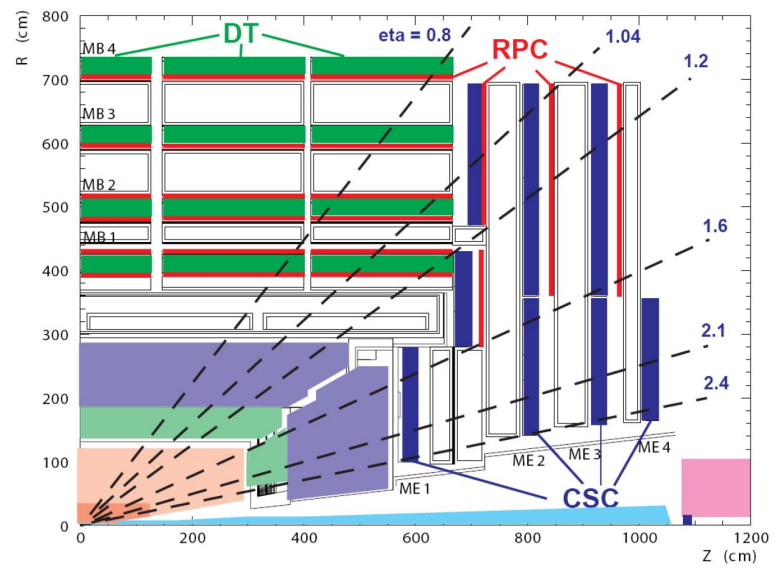
\includegraphics[width=0.7\linewidth]{Figures/chapter2_Figure/MS_layout.png}
\caption{CMS muon system layout.}
\label{Fig:CMS_muon_system_layout}
\end{center}
\end{figure} 

\subsubsection{Drift Tubes of muon system of CMS}
The DTs are planted in the barrel region of CMS muon system that provides pseudorapidity coverage of $|\eta| < 1.2 $ as illustrated
in Figure \ref{Fig:CMS_muon_system_layout}. Whole DT system consists of 5 wheels 
along z-axis, and 4 stations along radial direction (MB1, MB2, MB3, MB4). Each station is build with 12 chambers except fourth which contains 14 chambers. Each drift
chamber of an average size of 2m$\times$2.5m  is made of 12 aluminium layers, making 3 groups of four. The central group provides the coordinates 
measurement along z-axis and other two groups measures $r-\phi$. There are about 60 drift tubes in each chamber, each 4~cm wide made of drift cells each
of size 42~mm~$\times$~13~mm. The 50$\mu$m wire made of stainless steel serves as anode while two ``I-shaped`` aluminum tape each of thickness 50$\mu$m 
are  cathodes of the drift cell as shown in Figure \ref{Fig:CMS_DT_electric_field}. As any charges particle pass by the drift cell,  it ionizes the gas by 
removing electrons from its atom. This establish a electric field finishing of at positively charged wire.  Distance between the  wire and the muon 
track is estimated by drift time of these electrons.  The cell is filled with mixture of CO${}_{2}$ (15\%) Ar (85\%) gases which is 
inexpensive and safe. Other qualities of this mixture are good saturation drift velocity (5.4~cm/$\mu$s) and quenching. To keep 
drift velocity steady, the filled gas is kept at a constant pressure inside the chambers. The pressure in each wheel is continuously monitored by sensors. 
It is expected to inject 10\% new gas everyday.

\begin{figure}
\begin{center}
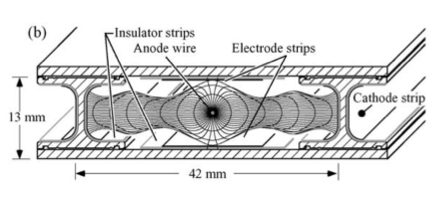
\includegraphics[width=0.7\linewidth]{Figures/chapter2_Figure/dt.png}
\caption{DT electric field created by cathode, anode and insulating strips .}
\label{Fig:CMS_DT_electric_field}
\end{center}
\end{figure} 
\subsubsection{Cathode Strip Chambers of the CMS muon system}
The cathode strip chambers (CSC) are installed at endcap region of CMS muon system providing the coverage of pseudorapidity upto $|0.9| < |\eta| < 2.4$, 
illustrated in Figure \ref{Fig:CMS_muon_system_layout}. In the endcap regions, the strength of magnetic field
 is non-uniform which forced to use in endcap some different technology from the barrel region. Another challenge for CSCs is  higher 
expected neutron-induced background as compared to the barrel region. The endcaps of the muon systems are made up of 468 CSCs arranged in four station like the
barrel region
(ME1, ME2, ME3 and ME4). The pseudorapidity range from $|0.9| < |\eta| < 1.2$ is covered by both CSCs and DTs. The chambers are aligned trapezoidal, each chamber
is covering 10${}^{\circ}$ or 20${}^{\circ}$ in $\phi$. RPCs are also installed between CSCs stations.
\par A single chamber is the basic unit which capable to work independently which is shown in Figure \ref{Fig:CMS_CSC_layout}. The CSC is multiple wire detector
made of 6 layers of positively 
charged anode interleaved with 7 layers of negatively charged cathode wires made of cooper filled within gas volume as shown in Figure \ref{Fig:CMS_CSC_layout}. The
cathode and 
anode wires are at right angle to each other and provides two position coordinates of each particle. As the charged particle pass through chamber, it will 
ionize the gas atoms producing avalanche of electrons to anode wires, illustrated in Figure \ref{Fig:CMS_CSC_layout_ef} . As the wires are 
nearby, CSCs not only provides excellent momentum resolution  but 
helps to trigger the event as well. It feeds $r-\phi$ resolution of 2~mm to first level trigger, $75\mu$m %off-line spatial resolution in $r-\phi$ 
for ME1/1 and ME1/2 chambers and $150\mu$m for other stations. The CSCs also help to assign bunch crossing with an efficiencies of 92\% which can be enhanced 
up to 99\% by simple majority out of all chambers. CSC has tendency to operate at high event rates and in an environment where the strength of magnetic field is non-uniform. This makes CSCs robust which does not require precise
gas pressure and temperature. Multilayer CSCs is useful for the combination of  hits in CSCs and tracker detectors.
%%%%%%
\begin{figure}[!htb]
  \begin{center}
    \subfigure[]{
      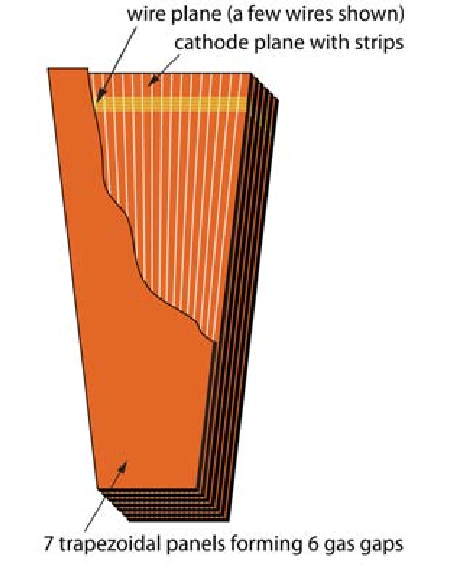
\includegraphics[width=0.48\textwidth,angle=0]{Figures/chapter2_Figure/csc_layout.png}
      \label{Fig:CMS_CSC_layout}
    }
    \subfigure[]{
      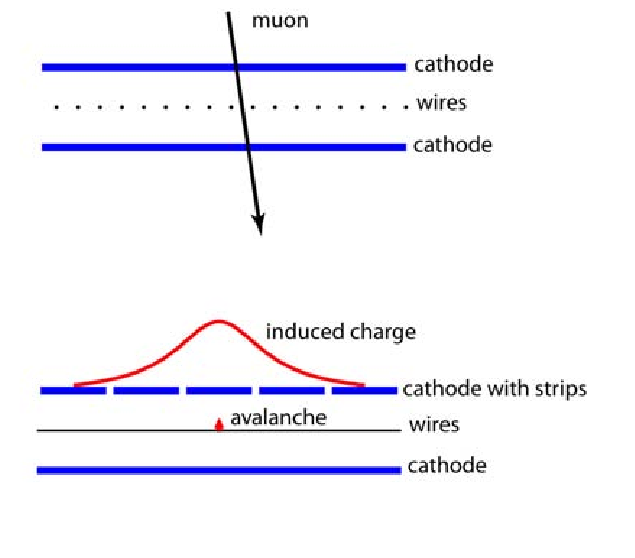
\includegraphics[width=0.48\textwidth,angle=0]{Figures/chapter2_Figure/csc_principle.png}
      \label{Fig:CMS_CSC_layout_ef}
    } 
    \caption{CSC layout (left) and induced current (right) when a charged particle pass thorugh it .}
  \label{fig:CSC_test_2}
\end{center}
\end{figure}

%=============
%============
\subsubsection{Resistive Plate Chambers of muon system of CMS}
RPCs are important part of CMS muon system installed in both barrel and endcap region. Time resolution of RPCs is excellent which is their main motivation. Additionally, spatial resolution of RPCs is also good. These  very fast responsive detector providing another muon trigger along with CSCs and DTs. RPCs are capable to provide 
a time resolution of about a nano-second.
\par RPCs are made of two high resistive plastic positive and negative charged plates, kept parallel to each other, with gas filled inn between them. The 
gas mixture consists of 95\% of $C_{2}H_{2}F_{4}$ and 5\% of $C_{4}H_{10}$. As the muon pass through the RPCs, electrons librated during primary and secondary ionization of the gas  create
avalanche which is received by outer metallic strips with a short but precise delay in time. Quick momentum measurement is feeded to trigger the event. The RPCs excellent time resolution assign bunch crossing 
with ultimate precision.
\subsubsection{Momentum Resolution}
CMS detector is capable to measure muons transverse momentum independently by  using tracker or muon system. The expected transverse momentum resolution of muons system
has been studied for the using muons of $p_{T} = 40$~GeV from Z and W boson decays and found to be 10\%(20\%) in barrel and endcap regions. Global muons can 
also be reconstructed at CMS by the combining the information from tracker and muons system. As compared to muon system, tracker gives better resolution for muons $p_T$ less than 100~GeV and vice versa. The transverse momentum resolution is found to be improved sufficiently by using global 
muons i.e 1\%(2\%) for $p_{T} < 100$~GeV in barrel(endcap) regions.
For muons with $p_{T}$  greatar than 100~GeV, transverse momentum resolution of CMS muon system improves upto 8\% and 10\% in the barrel and endcap regions respectively. 
Momentum 
resolution of CMS muon system alone, tracker alone and combination of both are shown in Figure \ref{Fig:CMS_muon_momentum_resolution}~\cite{cms:muonsystem_TDR_2}.
\begin{figure}
\begin{center}
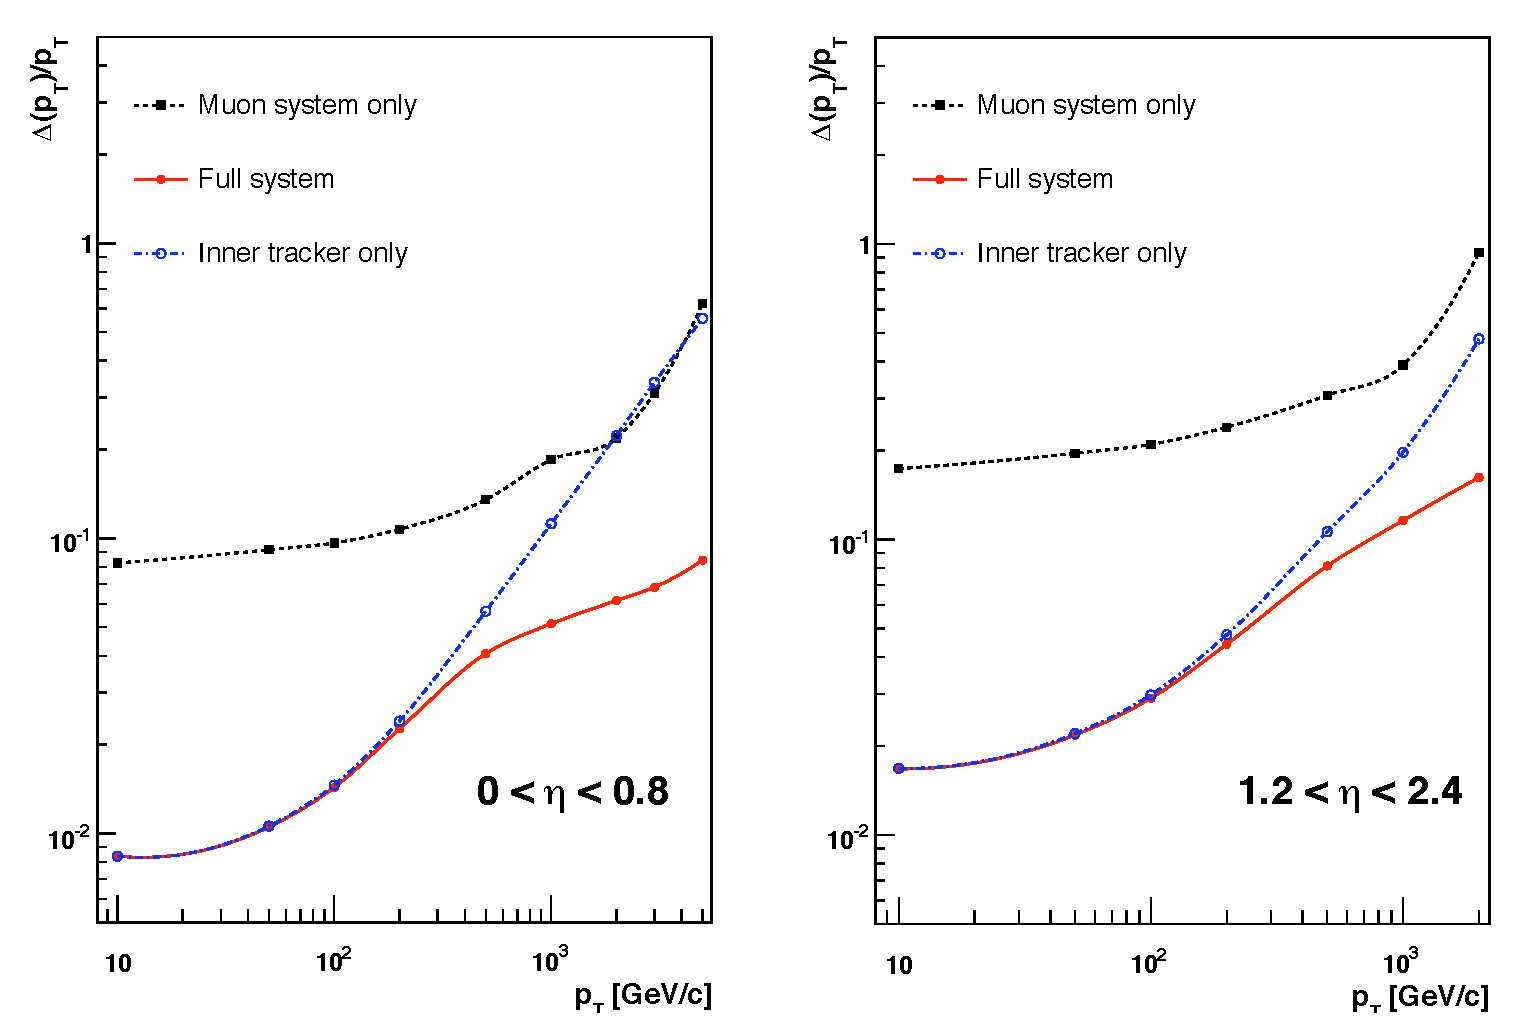
\includegraphics[width=0.7\linewidth]{Figures/chapter2_Figure/muon_resol.pdf}
\caption{Momentum resolution of muon as a function of $p_T$ of muons both in barrel and endcap regions.}
\label{Fig:CMS_muon_momentum_resolution}
\end{center}
\end{figure} 
\subsection{Trigger and Data Acquisition System of CMS}
The LHC running at its nominal parameters provides particle collisions produced with frequency of 40~MHz. Most of these events are soft collisions and uninteresting for new physics as they 
are like minimum bias collisions. Though CMS detector is capable to reconstruct all of these events but storing all these events will fill the CMS storage in days. 
So trigger system of CMS helps of select interesting events out of all for further steps. The events which does not pass the first step trigger are deleted permanently. 
Trigger system performs the first step for physics event selection which reduces the event rate from  40~MHz down to ~1kHz into two layers Level-1 and the high-level
triggers (shortly written as L1 and HLT respectively).
\par The L1 trigger is made of the programmable electronics, dropping the event rate drastically to 100~kHz. To be fast, L1 trigger events by their energy and momentum calculations
estimated by only using coarse in muon system and calorimeter instead of complete high resolution information. The L1 trigger decides to select or reject event in 3.2$\mu$m.   
\par All events with positive L1 decision, with their complete information, are transferred to HLT which makes use of one thousand commercial processors. It uses
the growing complex algorithms which exploit high details of the event. Decision time of HLT varies with event number with mean time of about $50$~ms. 
Since HLT has excess of complete information of an event, it demands a greater bandwidth of the order of 1Tb/s.
\par For example, to look for Higgs boson decay into 4-leptons final state, the trigger would look for energetic leptons in the detector. For L1 trigger, electron and muons 
points to a narrow energy deposit in ECAL and hit pattern in tracker and the muon system respectively. While for HLT, momentum and total energy of the leptons 
are reconstructed by ECAL and combination of muon system and inner tracker.
\subsubsection{Level-1 Trigger Architecture}
Configuration of L1 trigger is elaborated in Figure \ref{Fig:CMS_L1_trigger_configuration}. It can be classified into calorimeter 
and muon triggers. Each ECAL and HCAL has independent regional trigger feeding to global calorimeter trigger. Similarly, muon 
trigger has local triggers for each sub-detector merging into global muon trigger. Finally, global calorimeter and muon triggers merge into global trigger which
makes L1 final decision.
\par Each local trigger feeds to global/regional trigger by providing trigger primitives groups (TPGs) based on coarse of sub-detector. Regional calorimeter trigger (RCT)
 builds objects which deposit their energy in ECAL and HCAL such as jets, $\gamma$, electrons, photons and tau's.  Similarly, in muon triggering, DT/CSC/RPC track finders
 feeds muons tracks to muon global trigger (MGT). Global muon and calorimeter trigger feeded four best candidates at most, which are then sent to global trigger (GT).
 GT compares these candidates with L1 trigger menu to decide weather to keep to reject the event. Some triggers in the  menu evolved  with increasing LHC center
 of mass energy by tightening the requirement on candidate or  pre-scaled (selecting only the nth event) to control the output rate. Candidates 
 able to fire at least one trigger out of whole trigger menu is kept for further investigation by HLT. For example, the trigger/bit ``L1 SingleEG8Iso'' in the L1 trigger 
 menu requires one isolated (candidate with zero or little hadronic activity around it) electron or photon at least with $p_{T}$ greater than 8~GeV. 
\begin{figure}
\begin{center}
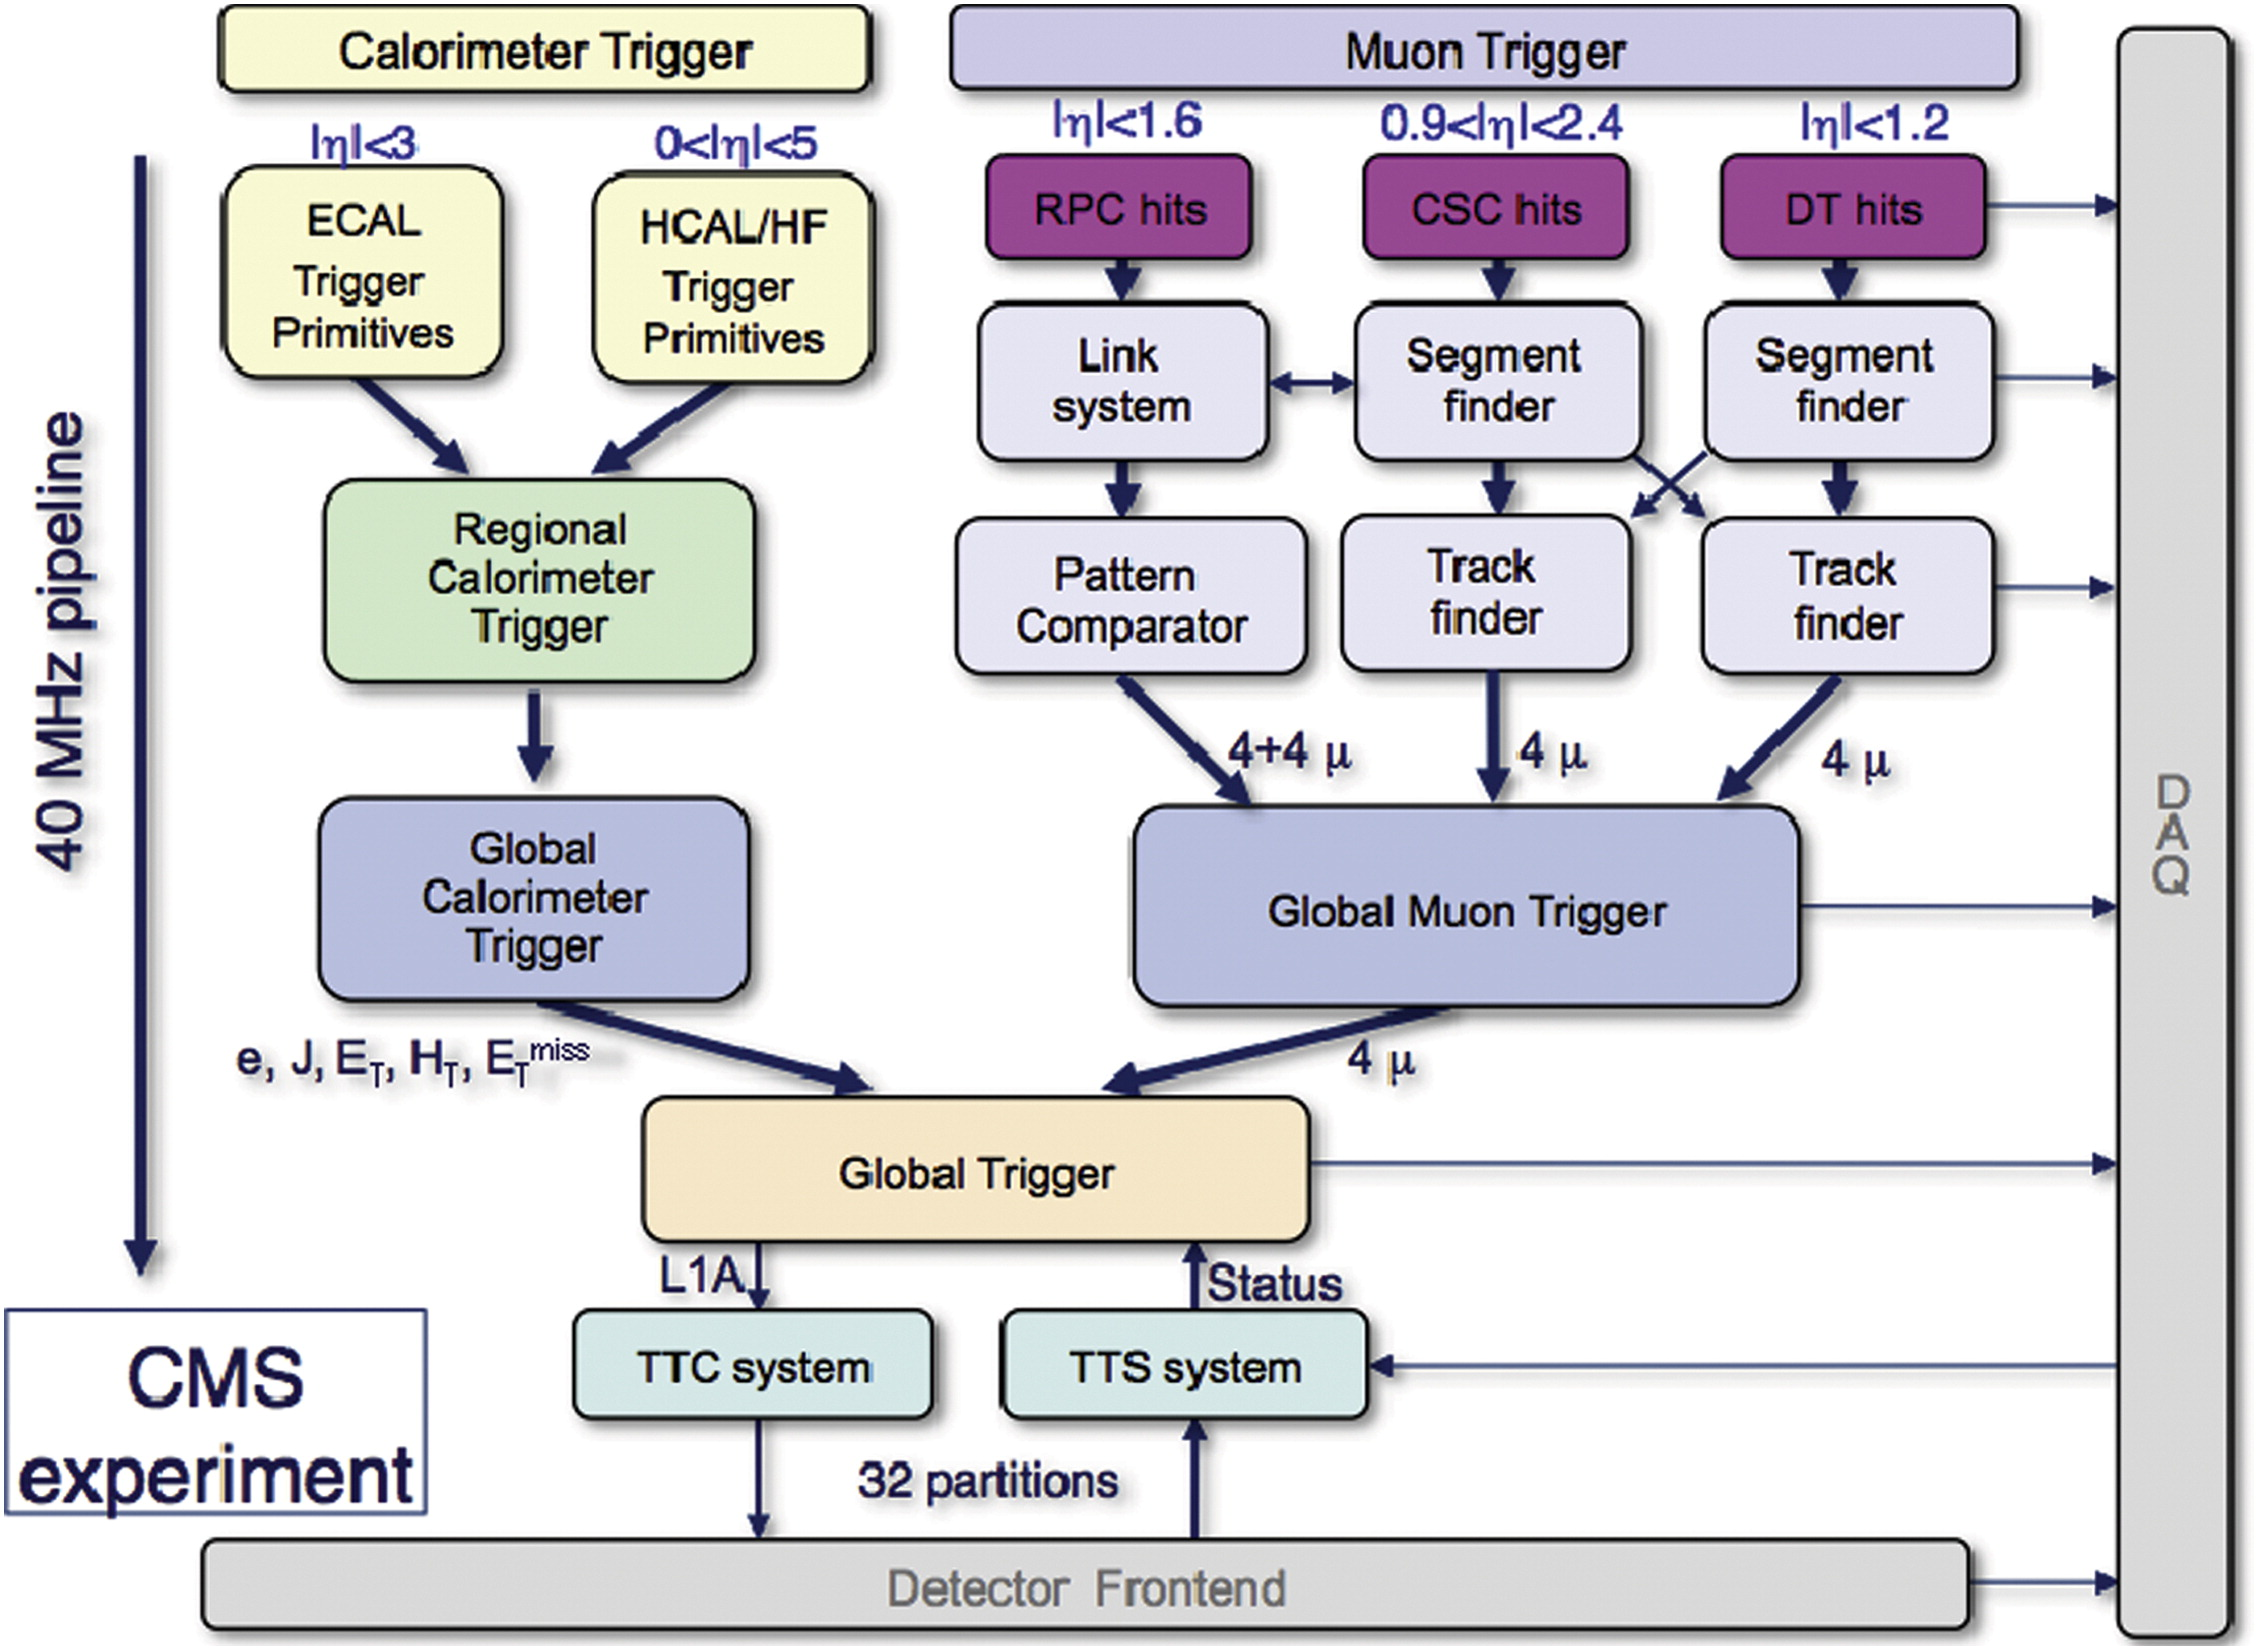
\includegraphics[width=0.7\linewidth]{Figures/chapter2_Figure/L1_new.jpg}
\caption{The configuration of L1 trigger.}
\label{Fig:CMS_L1_trigger_configuration}
\end{center}
\end{figure} 
\subsubsection{High-Level Trigger Architecture}
HLT  is three level (2, 2.5 and 3) trigger with growing complexity starting at level 2  which usually works on top of the information provided by L1 trigger. Goal of the HLT is to use output event rate of L1-trigger(100kHz) and reduce it upto 1 kHZ.  Level 2 HLT is to build fine granularity objects by combining the information from sub-detectors e.g from preshower and ECAL energy clusters are combined for electrons. Bremsstrahlung  
of the electrons causes its energy to spread into several neighbor cells. To compensate this effect, clusters of ECAL are combined to form superclusters.
\par At HLT level 2.5, the inner tracker information is combined and matched with calorimeters and muon system. In case of electron, energy supercluster is 
matched with the hits in the tracker, if matches it form a seed. Tracker hits are matched with the hits in muon system to reconstruct global muon.
HLT level 3 reconstructs the complete track, if its found electron seed or matching hits of muon. After these three stages, precise energy and momentum are calculated of 
the objects that decides to accept or reject the event. 
\par There are more than 200 different HLT paths each derived by at least one L1 bit. The data which pass the HLT trigger is organized into different 
datasets according to the objects reconstructed in the event and the passed selection e.g an event with two muons reconstructed with transverse momentum
greater than 8 and 17~GeV will be placed in "DoubleMu'' dataset. 
\subsubsection{Data Acquisition (DAQ) System of CMS}
The schematic skeleton of CMS DAQ system is presented in Figure \ref{Fig:CMS_DAQ_layout}. CMS DAQ provides data from 650 different readout channels to 
HLT along with enough computing resources to limit the output data rate~\cite{cms:DAQ_TDR}. Frangments of an event with a size of 2KB is provided by each module. 
In order to read data from detector sensors, Front End Drivers (FEDs) utilizea network whose bandwidth is 100 Gb/s.  These FEDs are located underground
at the level of the detector called counting room. Events are then transferred to a system where these are filtered at 100 kHz rate maximum. The complete reconstruction
of the objects of the event and high machine luminosity is the reason for this high rate.
\begin{figure}
\begin{center}
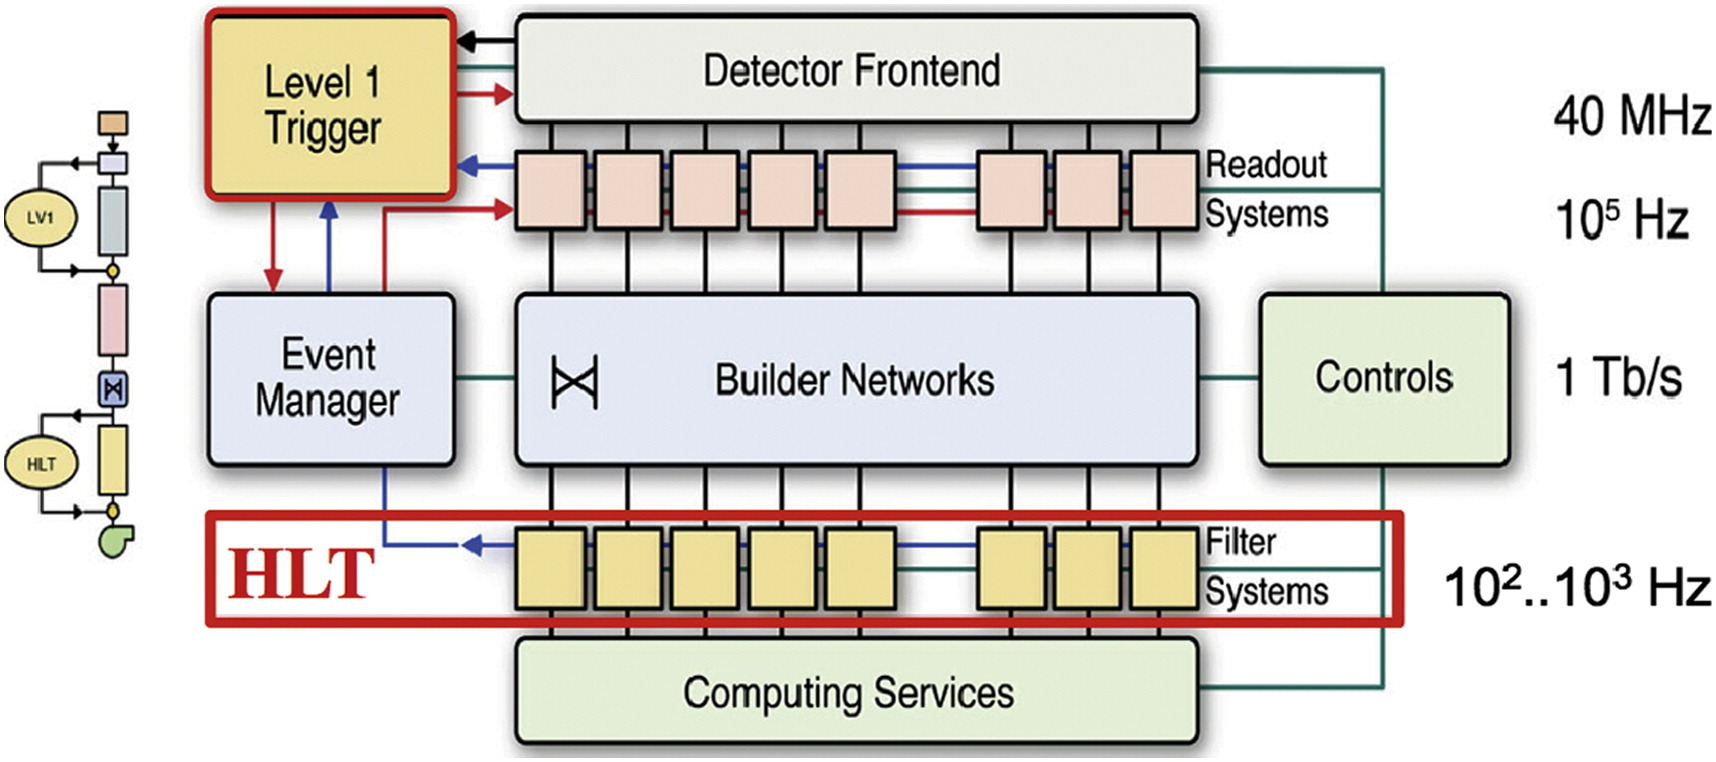
\includegraphics[width=0.7\linewidth]{Figures/chapter2_Figure/daq_new.jpg}
\caption{The CMS DAQ system structure.}
\label{Fig:CMS_DAQ_layout}
\end{center}
\end{figure}
\subsection{Computing Grid}
An important and last step after data collection is to process it with full detailed reconstruction algorithms and made available for physics analysis.Although,  
trigger system of CMS drastically reduces the amount of data but even then CMS delivers data at the order of petabytes every year.  To analyze and store this huge 
amount of the data, LHC has connected huge number of computing resources from collaborative institutes or universities, computer centers and middleware providers 
through a grid known as the Worldwide LHC Computing Grid (WLCG). 
\par There are three layers of Tier (Tier-0, Tier-1 and Tier-2) for data flow between different computing sites. 
The types of dataset is described below briefly
\begin{itemize}
 \item RAW data that contains all the recorded information from detector along with triggers decisions and other metadata. A copy of RAW data is achieved and placed
 at permanent storage element. A occupancy of  around 1.5 (2.0) MB/event is needed to store data (simulated data) in RAW version.
 \item Many algorithms and pattern recognition techniques like cluster and track-finding; primary and secondary vertex reconstruction etc. are applied to RAW data to 
 obtain RECO data format. RECO events occupancy is roughly three times less than RAW (0.5~MB/event).
 \item The most compact format of data AOD (analysis object data) is obtained by dropping unnecessary information and reducing per event size up to 100 KB.
\end{itemize}
Tier-0 is located at CERN with which copies the recorded data to permanent storage, promptly reconstruct data from RAW version to have first version of
prompt-RECO data and copies RAW data to Tier-1 centers. Tier-1 are mainly held in national computing centers and labs from collaborative countries. 
At each Tier-1, a fraction of detailed the reconstruction of RAW data simulated data has been performed to get AOD. Tier-1 also responsible to store and 
export AOD format data to Tier-2. The last layer Tier-3 is hosted by CMS collaborative institutes where main analysis activity, alignment, detector related studies and 
offline calibration is done. Tier-3 are used for Monte Carlo (MC) data production which can be exported to Tier-1 for long term storage.
